\documentclass[a4paper,12pt]{book}

\usepackage{polski}
\usepackage[utf8]{inputenc}
\usepackage[polish]{babel}
\usepackage[unicode]{hyperref}
\usepackage{tabto}
\usepackage{graphicx}
\usepackage{pythonhighlight}
\usepackage{amsmath}
\usepackage{float}

\hypersetup{
	colorlinks=true,
	linkcolor=blue,
	filecolor=magenta,      
	urlcolor=cyan,
}
\graphicspath{ {./images/} }

\title{\Large{\textbf{Przetwarzanie Obrazów: Sprawozdanie}}}
\author{
	Damian Ubowski
	\and
	Maciej Tarach
}
\date{Warszawa, 2019}

\begin{document}
\maketitle
\tableofcontents
\chapter{Wstęp}
\section{Format obrazu}
Wybranym przez nas formatem obrazów cyfrowych jest DjVu, który jest oparty na zaawansowanej metodzie segmentacji obrazu. Tworzenie pliku DjVu polega na rozdzieleniu dowolnie skomplikowanego obrazu na odrębne warstwy, a następnie poddaniu warst odrębnym optymalizacjom i kompresjom. Format ten stosuje ładowanie progresywne, kodowanie arytmetyczne, oraz kompresję stratną dzięki czemu przy minimalnej ilości przestrzeni dyskowej można delektować się obrazami i dokumentami w wysokiej jakości. 
\subsection{Struktura formatu}
Pliki DjVu rozpoczynają się od swojej ``Magic number'' potwierdzającej rodzaj pliku i mającej wartość \textit{0x41 0x54 0x26 0x54}. Następnie czerpiąc inspirację ze struktury IFF \textbf{(Interchange File Format)} plik dzieli się na kawałki (\textit{ang. chunks}) zawierające interesujące nas cenne dane. Takie jak szerokość lub wysokość obrazu, dpi, informacje o kolorach, rozmieszczeniu pikseli, etc. Każdy kawałek składając się z ID typu, długości zawartości i samej zawartości tworzy zwarty format. Identyfikator typu określa rolę w jakiej przyjdzie służyć kawałkowi. Do dyspozycji ma ich całkiem sporo, ale uwzględniając najbardziej przydatne w naszym kontekście to ograniczymy liczbę do: 
\renewcommand{\labelitemi}{$*$}
\begin{itemize}
	\item BGjp - warstwa tylna przechowywana przy użyciu kodowania JPEG. 
	\item BFjp - warstwa przednia w formacie JPEG. 
	\item INFO - opisuje wysokość, szerokość, rozdzielczość, wersję kodera, oraz flagi wskazujące na obrót obrazu. 
\end{itemize}
\subsection{Przykładowa struktura IFF}
FORM:DJVU [14260] \newline
\tabto{5mm} INFO [10] \newline
\tabto{5mm} Sjbz [13133] \newline
\tabto{5mm} FG44 [181] \newline
\tabto{5mm} BG44 [935] \newline
\newline
Powyższa struktura przedstawia dokument składający się z jednej strony, na co wskazuje \textit{FORM:DJVU}, wraz z grafiką. Ten znacznik informuje, że mamy do czynienia z kontenerem o długości 14260 bajtów, który może zawierać inne kawałki dokumentu. Zgodnie z konwencją, po identyfikatorze typu i informacji o długości znajduje się zawartość kawałka. W tym wypadku jak i w każdym innym po \textit{FORM:DJVU} powinno znaleźć się \textit{INFO} z podstawowymi informacjami. Jeśli konwencji i wymagań specyfikacyjnych stało się zadość wtedy czas nastał na jakieś wizualne atrakcje takie jak \textit{Sjbz}, czyli masce wyboru pomiędzy kolorami z warstwy przedniej (\textit{FG44}) i tylnej (\textit{BG44}). 
\subsection{Instrukcja obsługi programu}
W celu uruchomienia kodu źródłowego będzie niezbędny: 
\begin{itemize}
	\item \href{http://djvu.sourceforge.net/}{DjVuLibre} ($\geq$ 3.5.21)
	\item \href{https://www.python.org/}{Python} ($\geq$ 2.6 lub 3.X)
	\item \href{https://cython.org/}{Cython} ($\geq$ 0.19, lub $\geq$ 0.20 dla Python 3)
	\item \href{https://wiki.freedesktop.org/www/Software/pkg-config/}{pkg-config} (POSIX)
\end{itemize}

\chapter{Operacje ujednolicania obrazów}
Ujednolicanie obrazów oznacza sprowadzenie ich do wspólnego gruntu pod względem określonego parametru. W tym wypadku będziemy ujednolicać obrazy pod względem geometrycznym (ilości kolumn i wierszy pikseli) i następnie rozdzielczościowym (wypełnienia pikselami). Sekwencyjność tych operacji jak i one same nie są w stanie spowodować spadku jakości obrazu. 
\section{Ujednolicenie obrazów szarych geometryczne}
\subsection*{Algorytm}
\subsubsection*{Opis}
Algorytm geometrycznego ujednolicenia obrazów ma za zadanie sprowadzić oba obrazy do tej samej liczby pikseli w każdym wierszu i każdej kolumnie. 
\subsubsection*{Kroki}
\begin{enumerate}
	\item Porównaj szerokości i wysokości obu obrazów i wybierz największe. 
	\item Jeśli pierwszy lub drugi obraz mają szerokość lub wysokość mniejszą od największej dostępnej to:
	\begin{enumerate}
		\item Utwórz czarne tło
		\item Przenieś z wyśrodkowaniem piksle na czarne tło
	\end{enumerate}
	\item Jeśli żaden z warunków jest niespełniony to nie rób nic
\end{enumerate}
\begin{figure}
	\caption{Przed uruchomieniem algorytmu (od lewej): obraz 1 (1067x1067, 300dpi), obraz 2 (2133x2133, 300dpi)}
	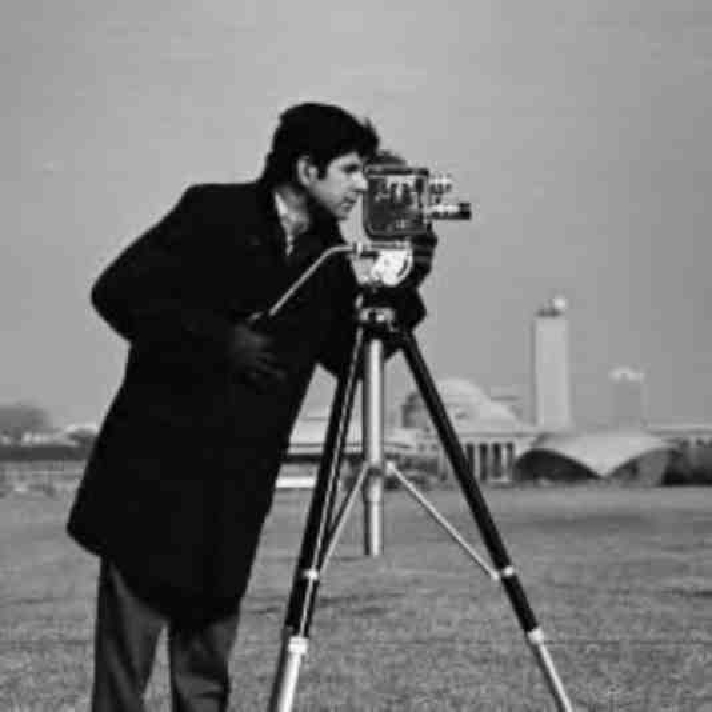
\includegraphics[width=8cm, height=8cm]{man-unmodified.jpg}
	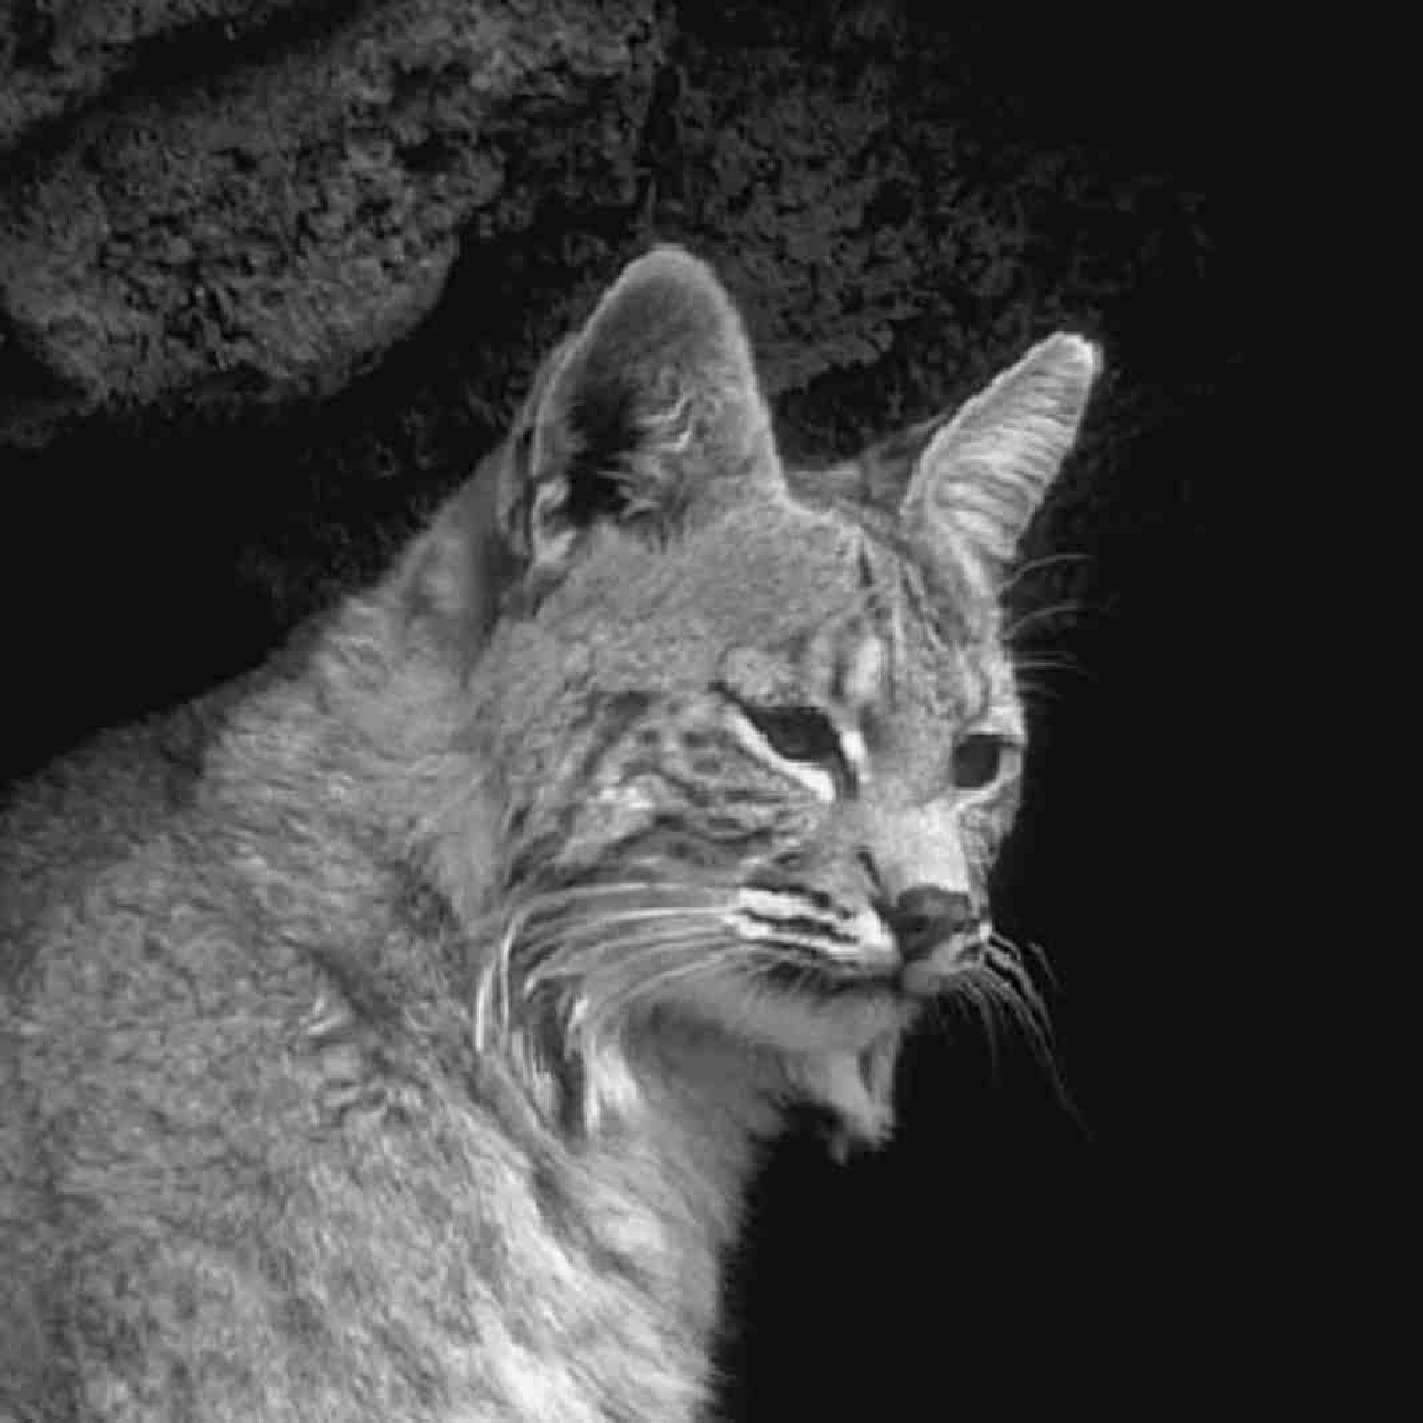
\includegraphics[width=8cm, height=8cm]{cat-unmodified.jpg}
\end{figure}
\begin{figure}
	\caption{Po uruchomieniem algorytmu (od lewej): obraz 1 (2133x2133, 300dpi), obraz 2 (2133x2133, 300dpi)}
	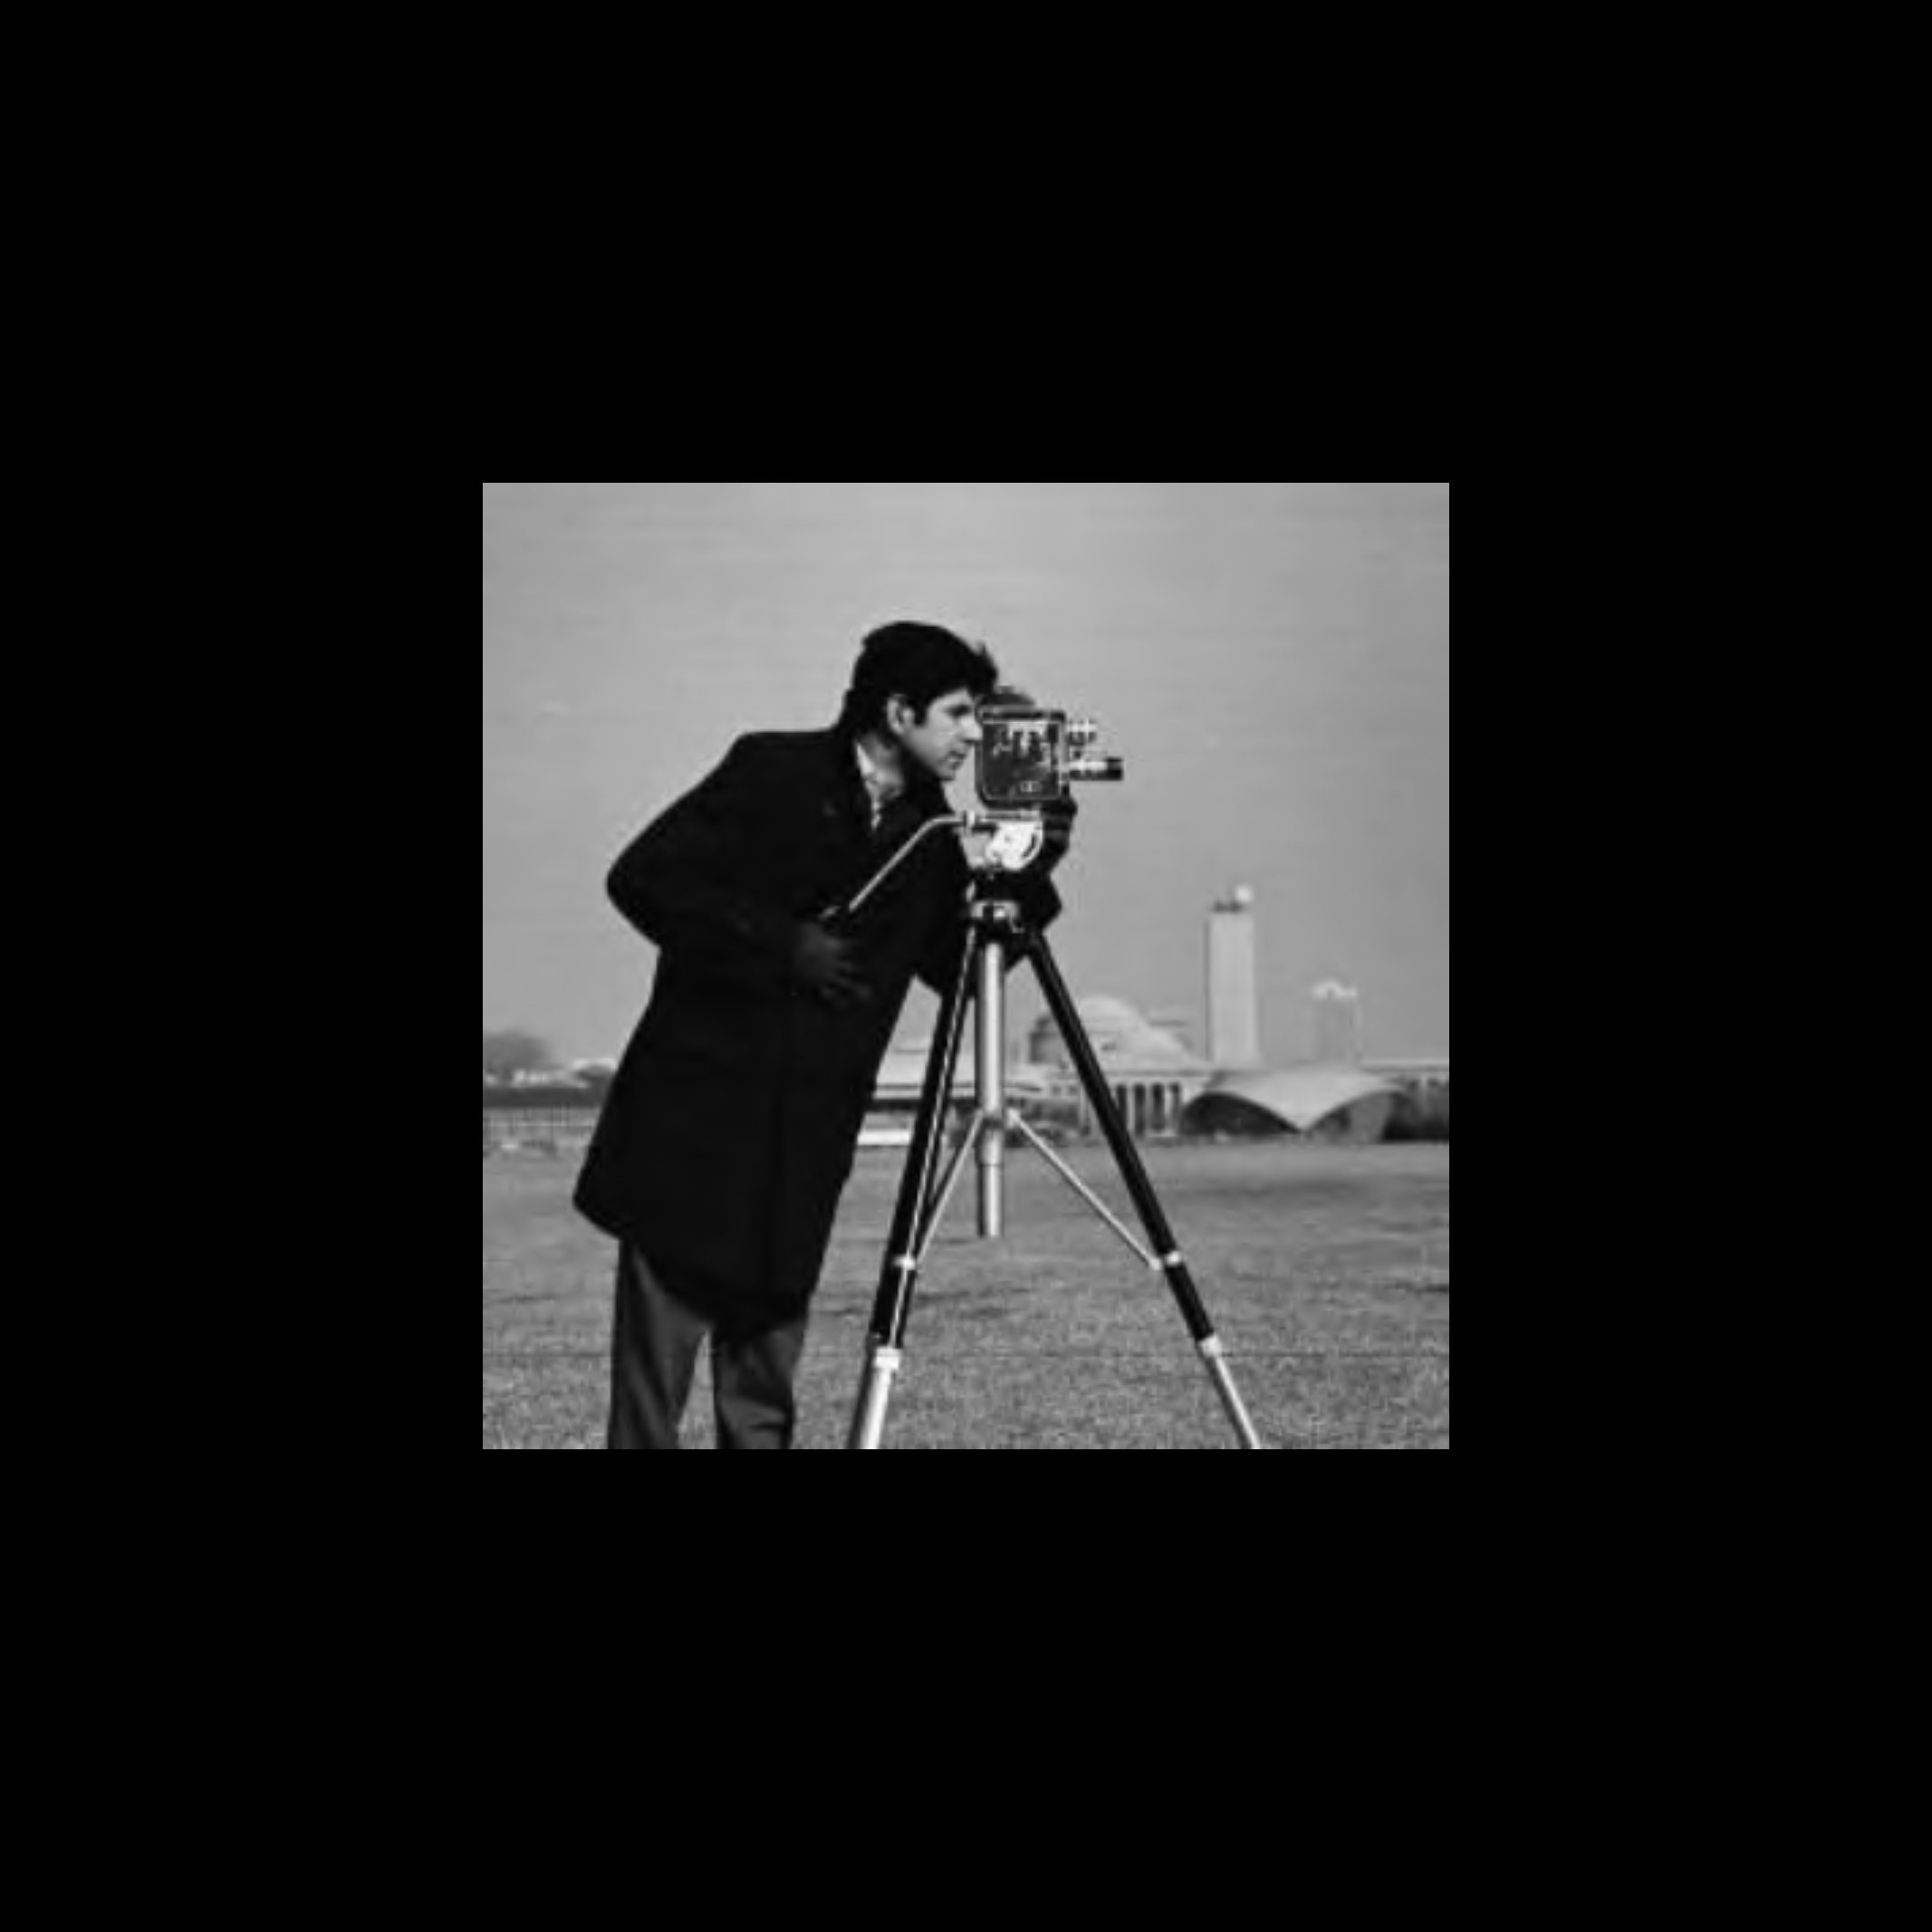
\includegraphics[width=8cm, height=8cm]{man-modified.png}
	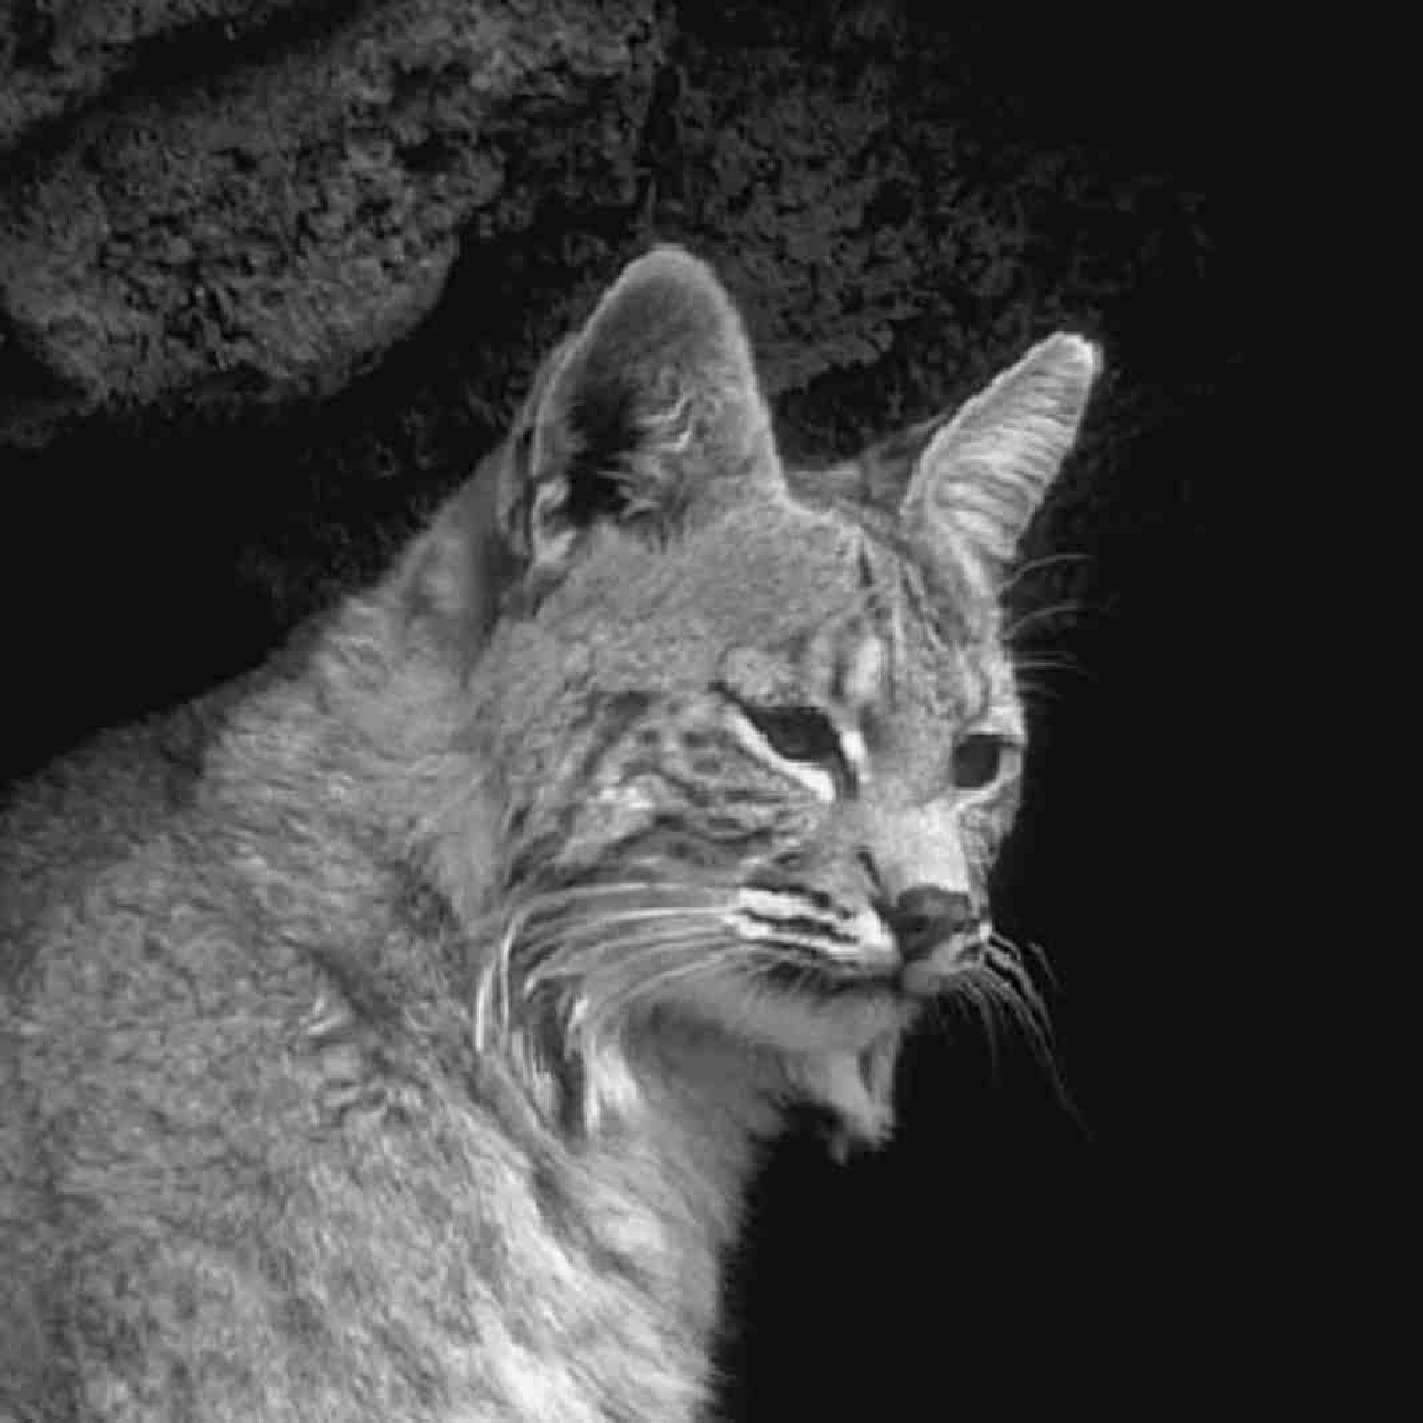
\includegraphics[width=8cm, height=8cm]{cat-unmodified.jpg}
\end{figure}
\subsection*{Kod źródłowy algorytmu}
\begin{python}
def geometricGray(self):
	print('geometric gray unificaiton start')
	width, height = self.firstDecoder.width, self.firstDecoder.height
	if width < self.maxWidth or height < self.maxHeight:
		# Create black background
		firstResult = numpy.zeros((self.maxHeight, self.maxWidth), numpy.uint8)
		# Copy smaller image to bigger
		startWidthIndex = int(round((self.maxWidth - width) / 2))
		startHeightIndex = int(round((self.maxHeight - height) / 2))
		pixelsBuffer = self.firstDecoder.getPixels()
		for h in range (0, height):
		for w in range (0, width):
		firstResult[h + startHeightIndex, w + startWidthIndex] = pixelsBuffer[h, w]
		img = Image.fromarray(firstResult, mode='L')
		img.save('Resources/ggUnification_1.png')
		print('first image done')
	
	width, height = self.secondDecoder.width, self.secondDecoder.height
	if width < self.maxWidth or height < self.maxHeight:
		# Create black background
		secondResult = numpy.zeros((self.maxHeight, self.maxWidth), numpy.uint8)
		# Copy smaller image to bigger
		startWidthIndex = int(round((self.maxWidth - width) / 2))
		startHeightIndex = int(round((self.maxHeight - height) / 2))
		pixelsBuffer = self.secondDecoder.getPixels()
		for h in range (0, height):
		for w in range (0, width):
		secondResult[h + startHeightIndex, w + startWidthIndex] = pixelsBuffer[h, w]
		img = Image.fromarray(secondResult, mode='L')
		img.save('Resources/ggUnification_2.png')
		print('second image done')
	print('geometric gray unification done')
\end{python}
\section{Ujednolicenie obrazów szarych rozdzielczościowe}
\subsection*{Algorytm}
\subsubsection*{Opis}
Po użyciu ujednolicenia geometrycznego można użyć ujednolicenia rozdzielczościowego, które przeskaluje obraz z mniejszej postaci do większej dzięki czemu nie zostanie nam czarna ramka wokół obrazu. Wynikiem będzie większy obraz niż początkowo bez czarnego obwodu wokół. 
Mniejszy obraz można przeskalować do większych wymiarów przenosząc wszystkie piksele z uwzględnieniem luk pomiędzy nimi i następnie użycia interpolacji do zamazania tych luk. 
Interpolacja działa na zasadzie pobierania wartości z okolicznych pikseli i wyciągania z nich średniej, która posłuży jako baza koloru dla nowego piksela. 
\subsubsection*{Kroki}
\begin{enumerate}
	\item Ustalenie nowych wymiarów obrazu
	\item Obliczenie odległości pomiędzy pikselami (\textit{scaleFactoryH, scaleFactoryW})
	\item Naniesienie pikseli z mniejszego obrazu na większy z uwzględnieniem luk
	\item Interpolacja
\end{enumerate}
\begin{figure}
	\caption{Skutki braku interpolacji}
	\begin{center}
		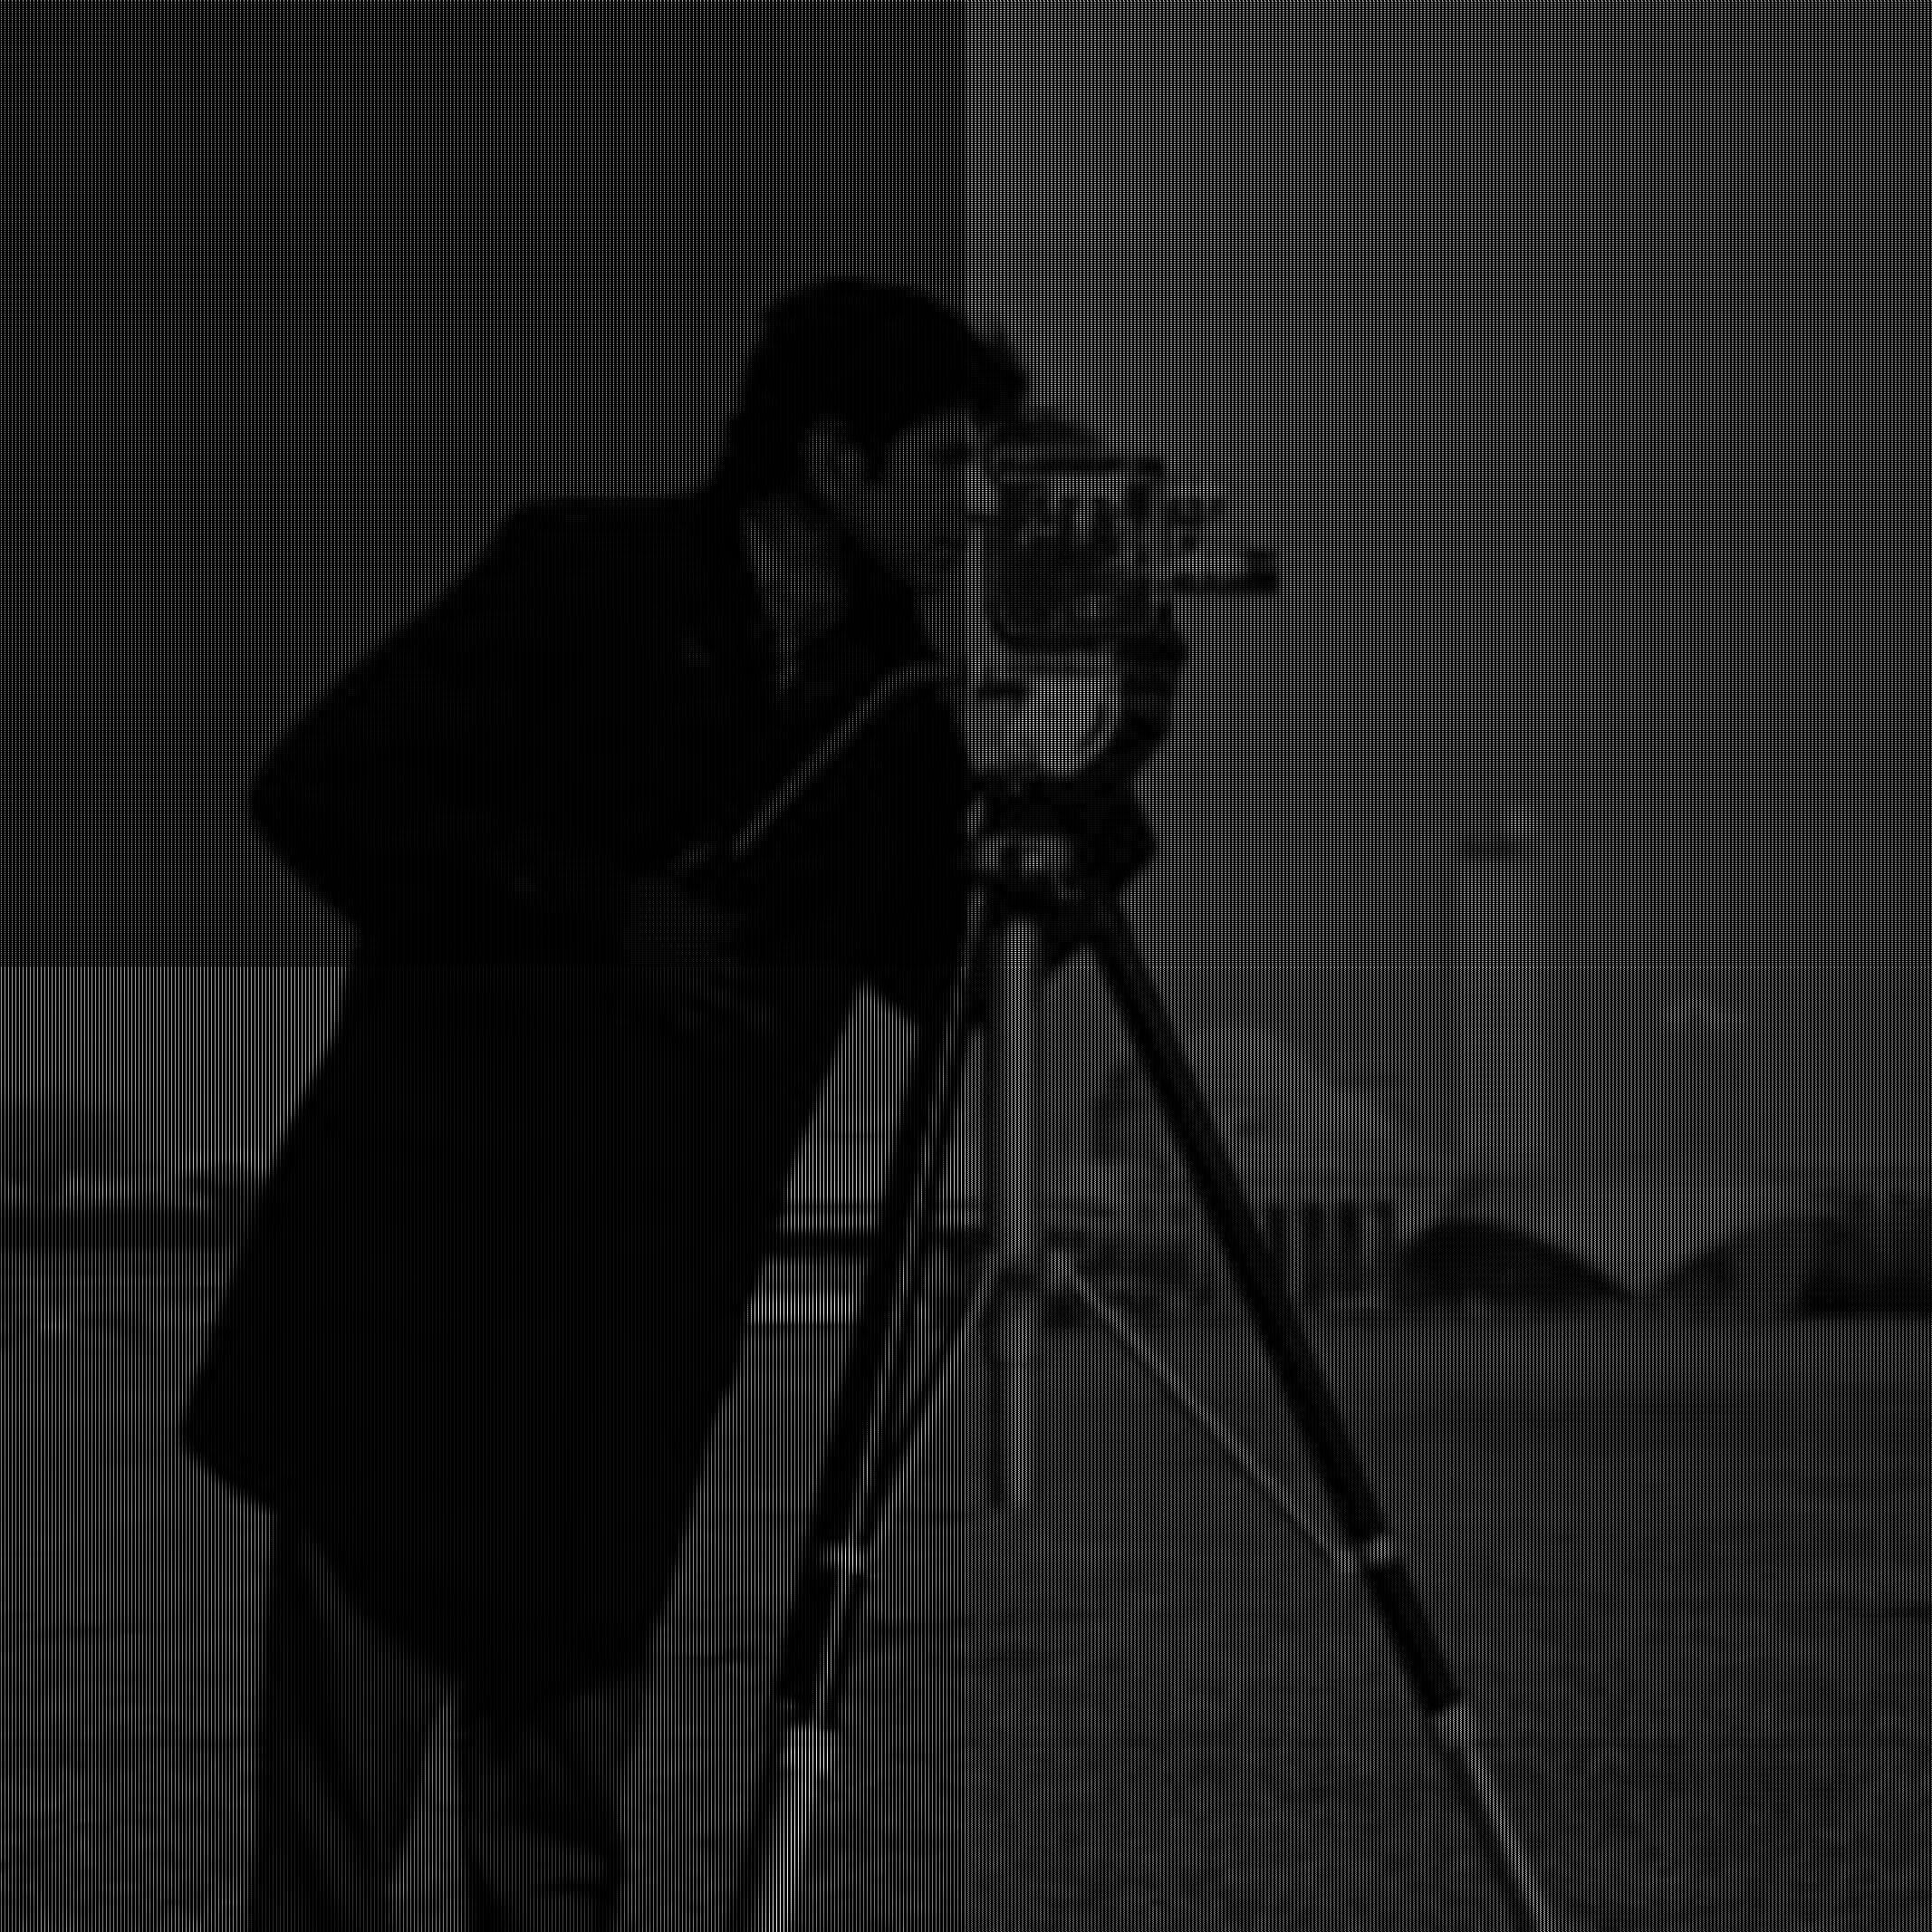
\includegraphics[width=8cm, height=8cm]{man-without-interpolation.png}
	\end{center}
\end{figure}
\begin{figure}
	\caption{Przed uruchomieniem algorytmu (od lewej): obraz 1 (2133x2133, 300dpi), obraz 2 (2133x2133, 300dpi)}
	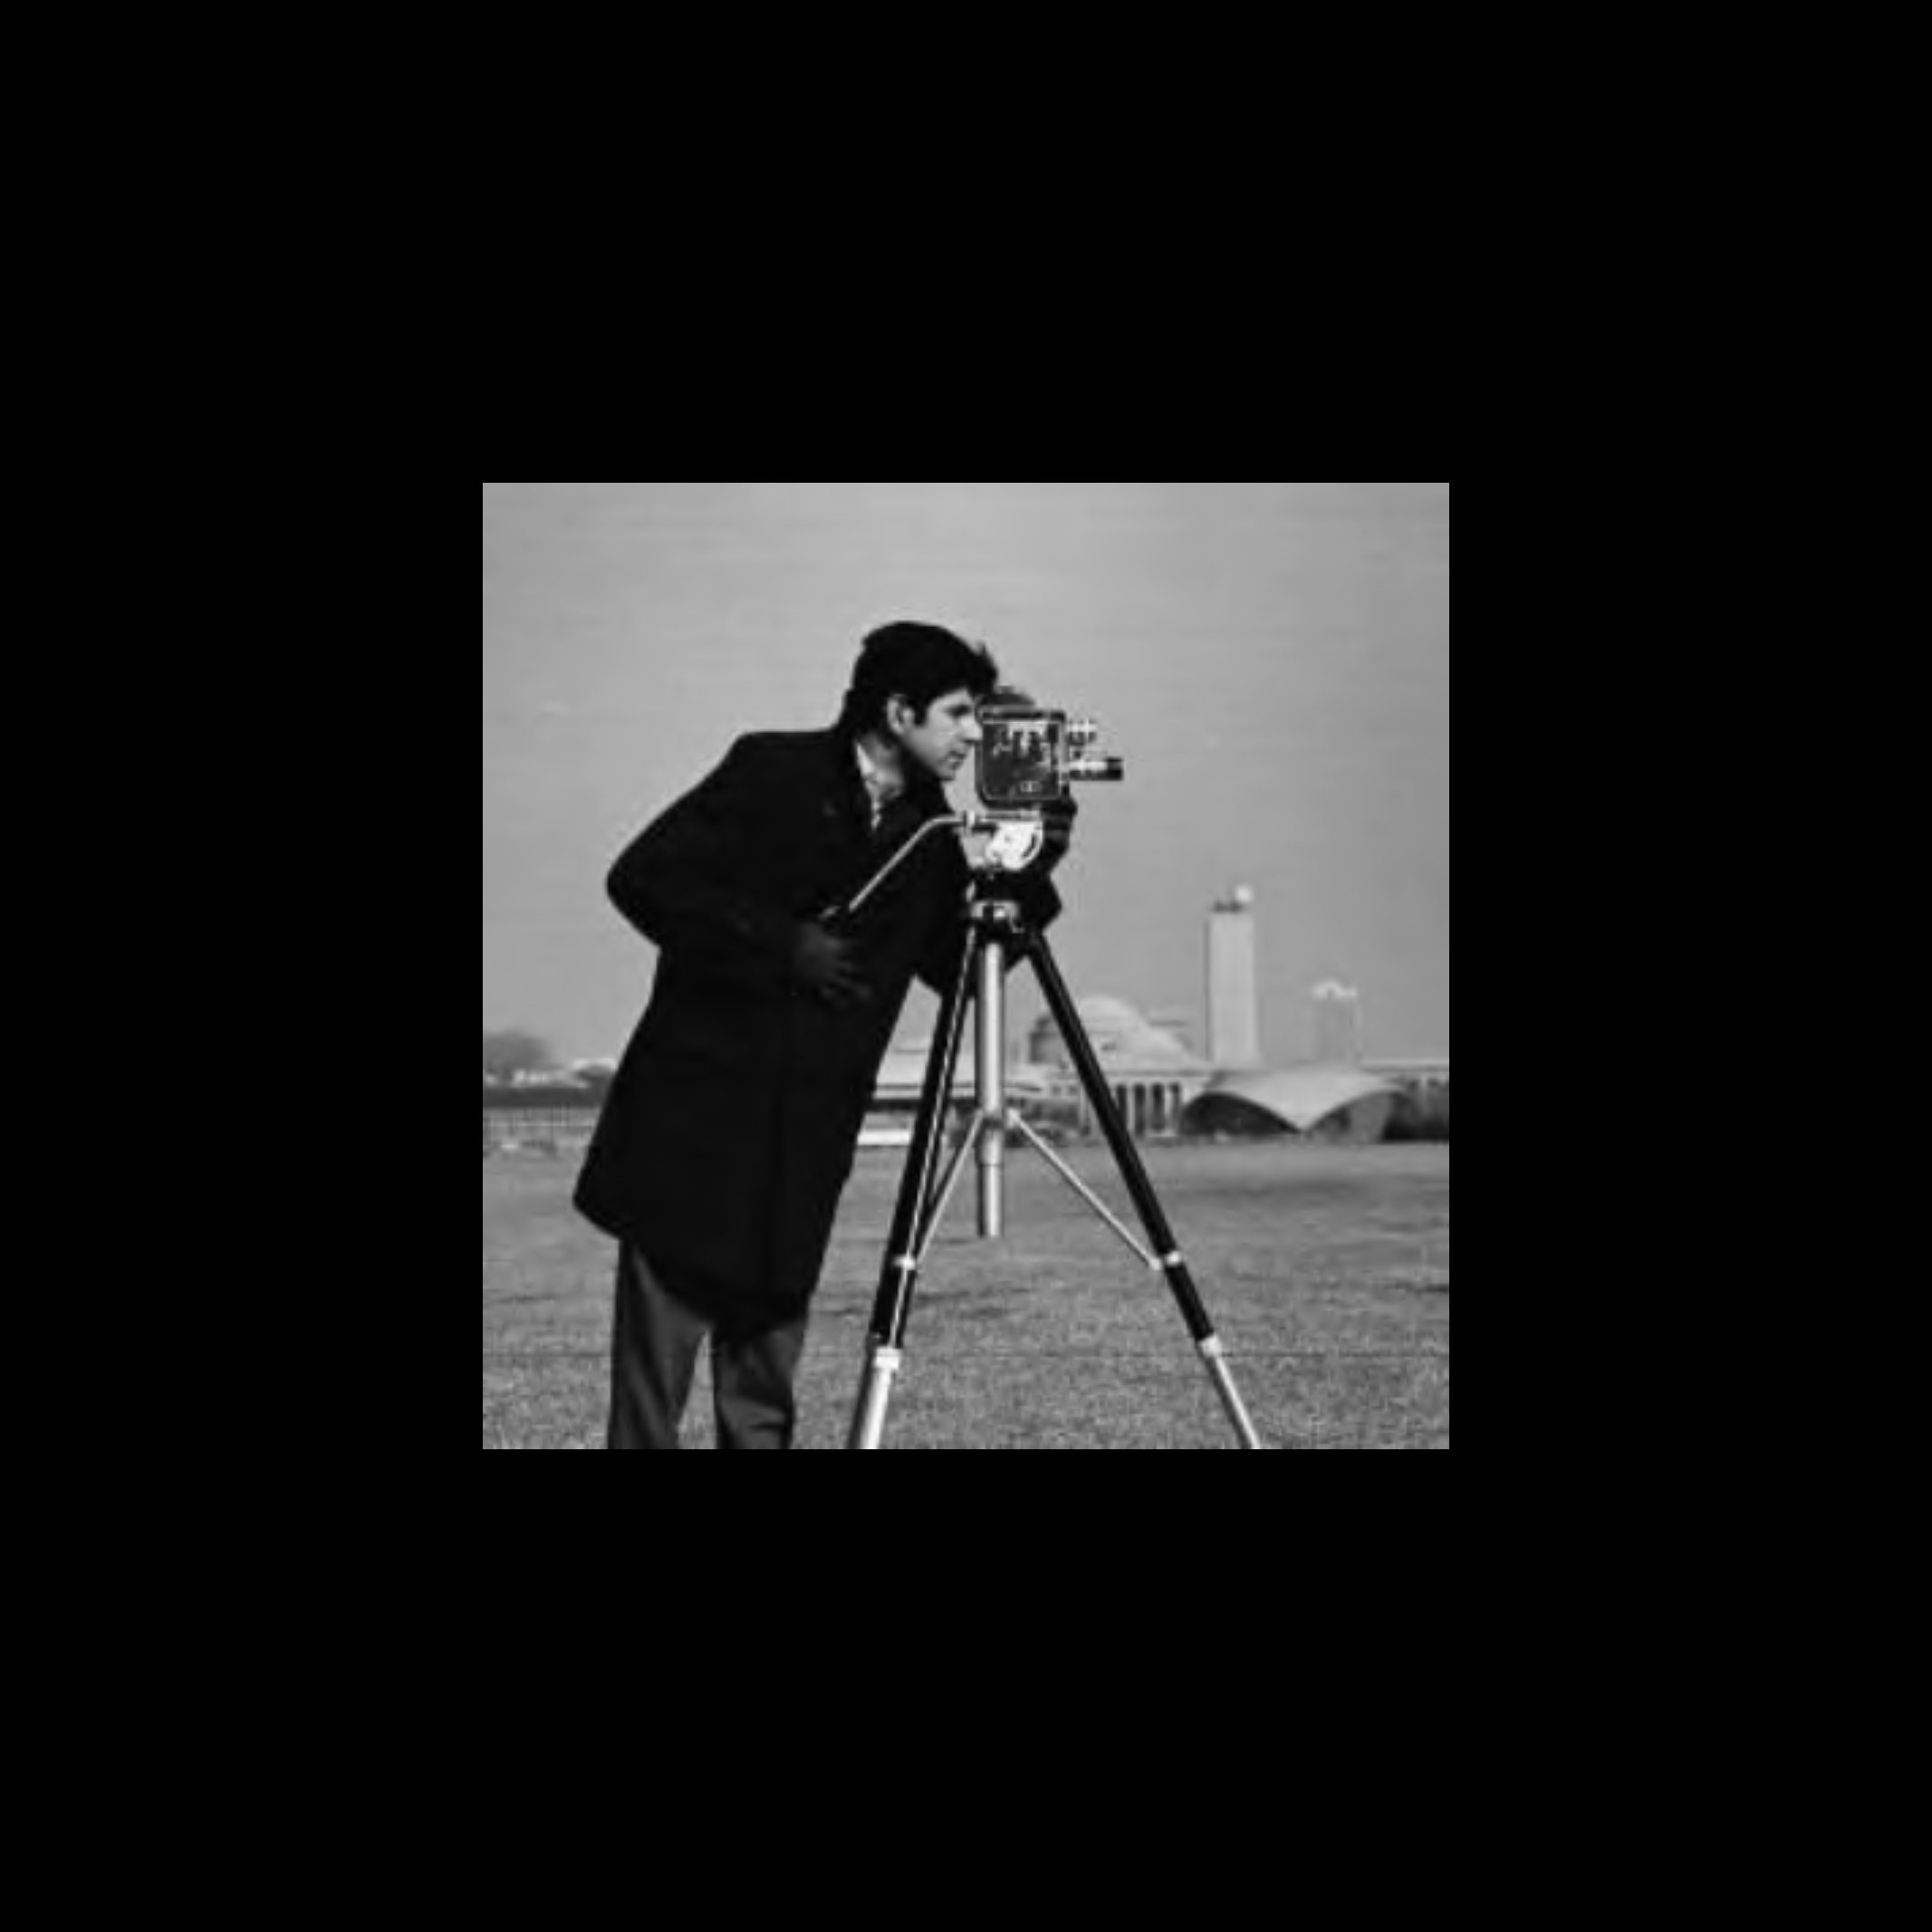
\includegraphics[width=8cm, height=8cm]{man-modified.png}
	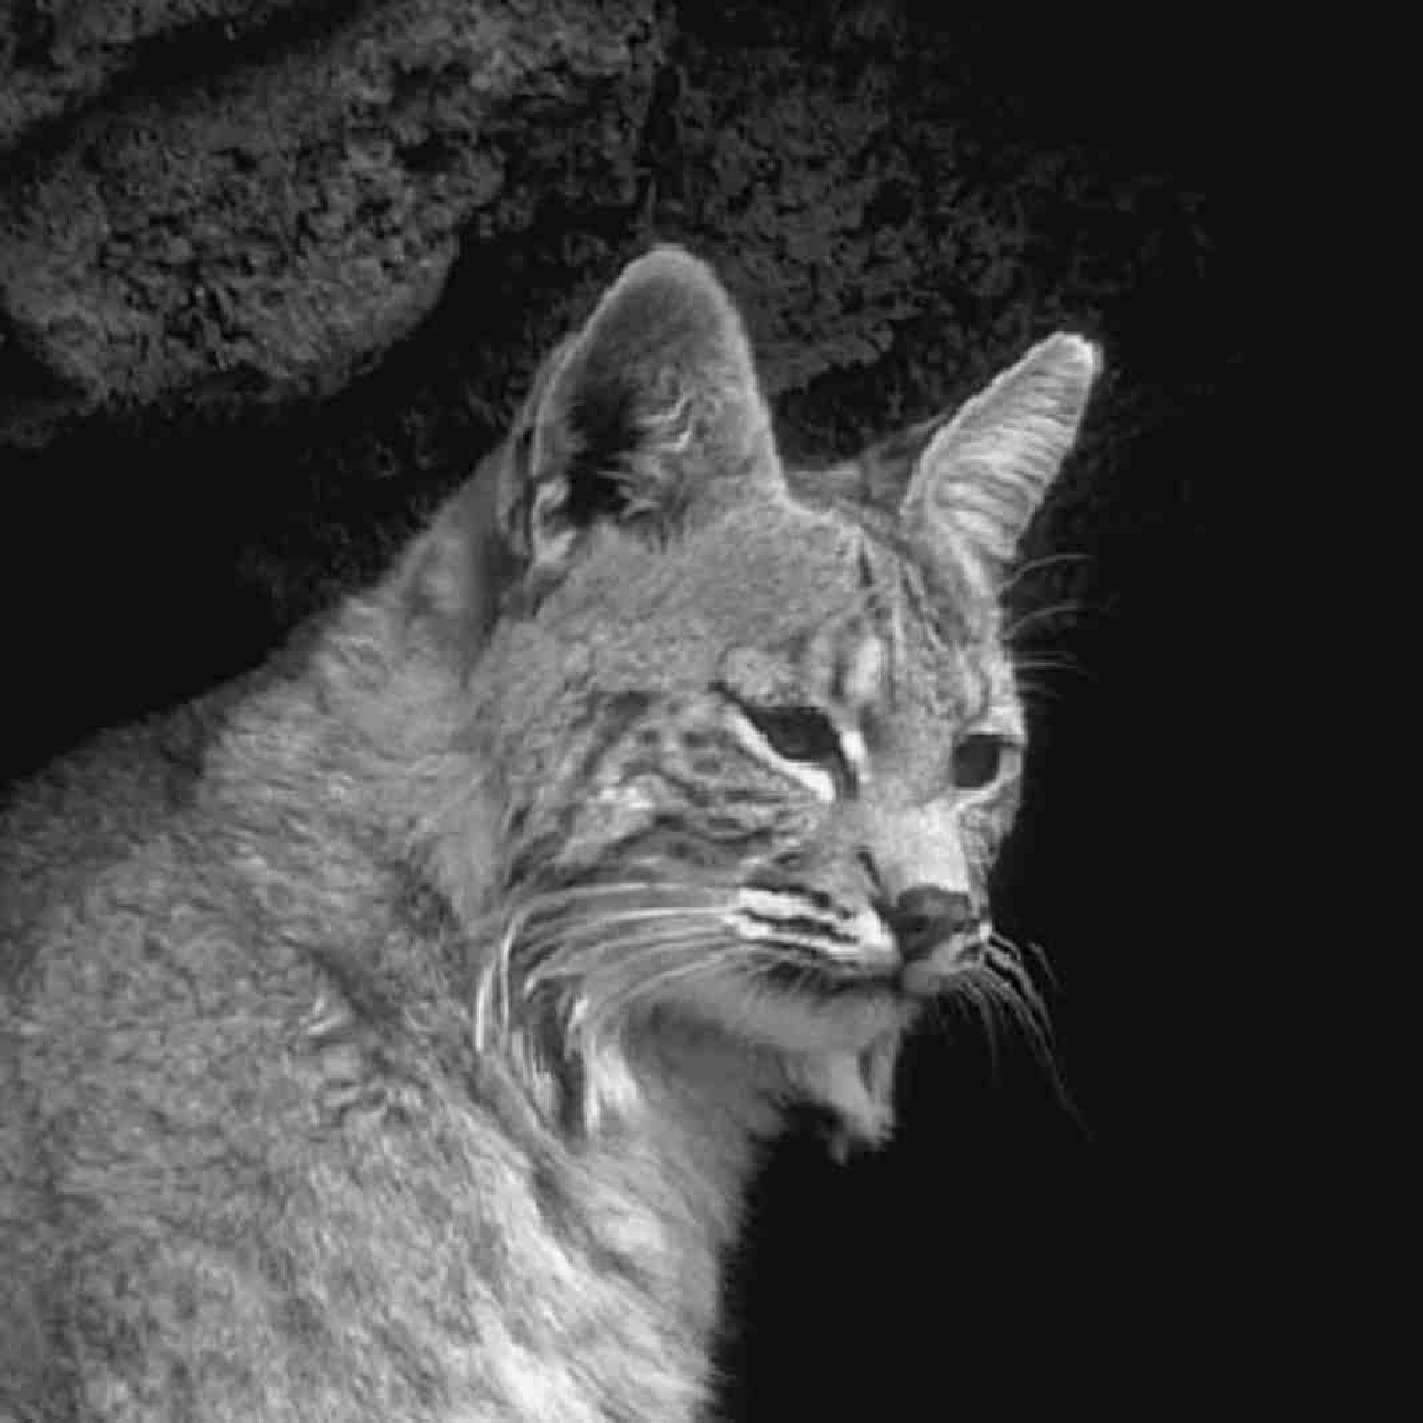
\includegraphics[width=8cm, height=8cm]{cat-unmodified.jpg}
\end{figure}
\begin{figure}
	\caption{Po uruchomieniem algorytmu (od lewej): obraz 1 (2133x2133, 300dpi), obraz 2 (2133x2133, 300dpi)}
	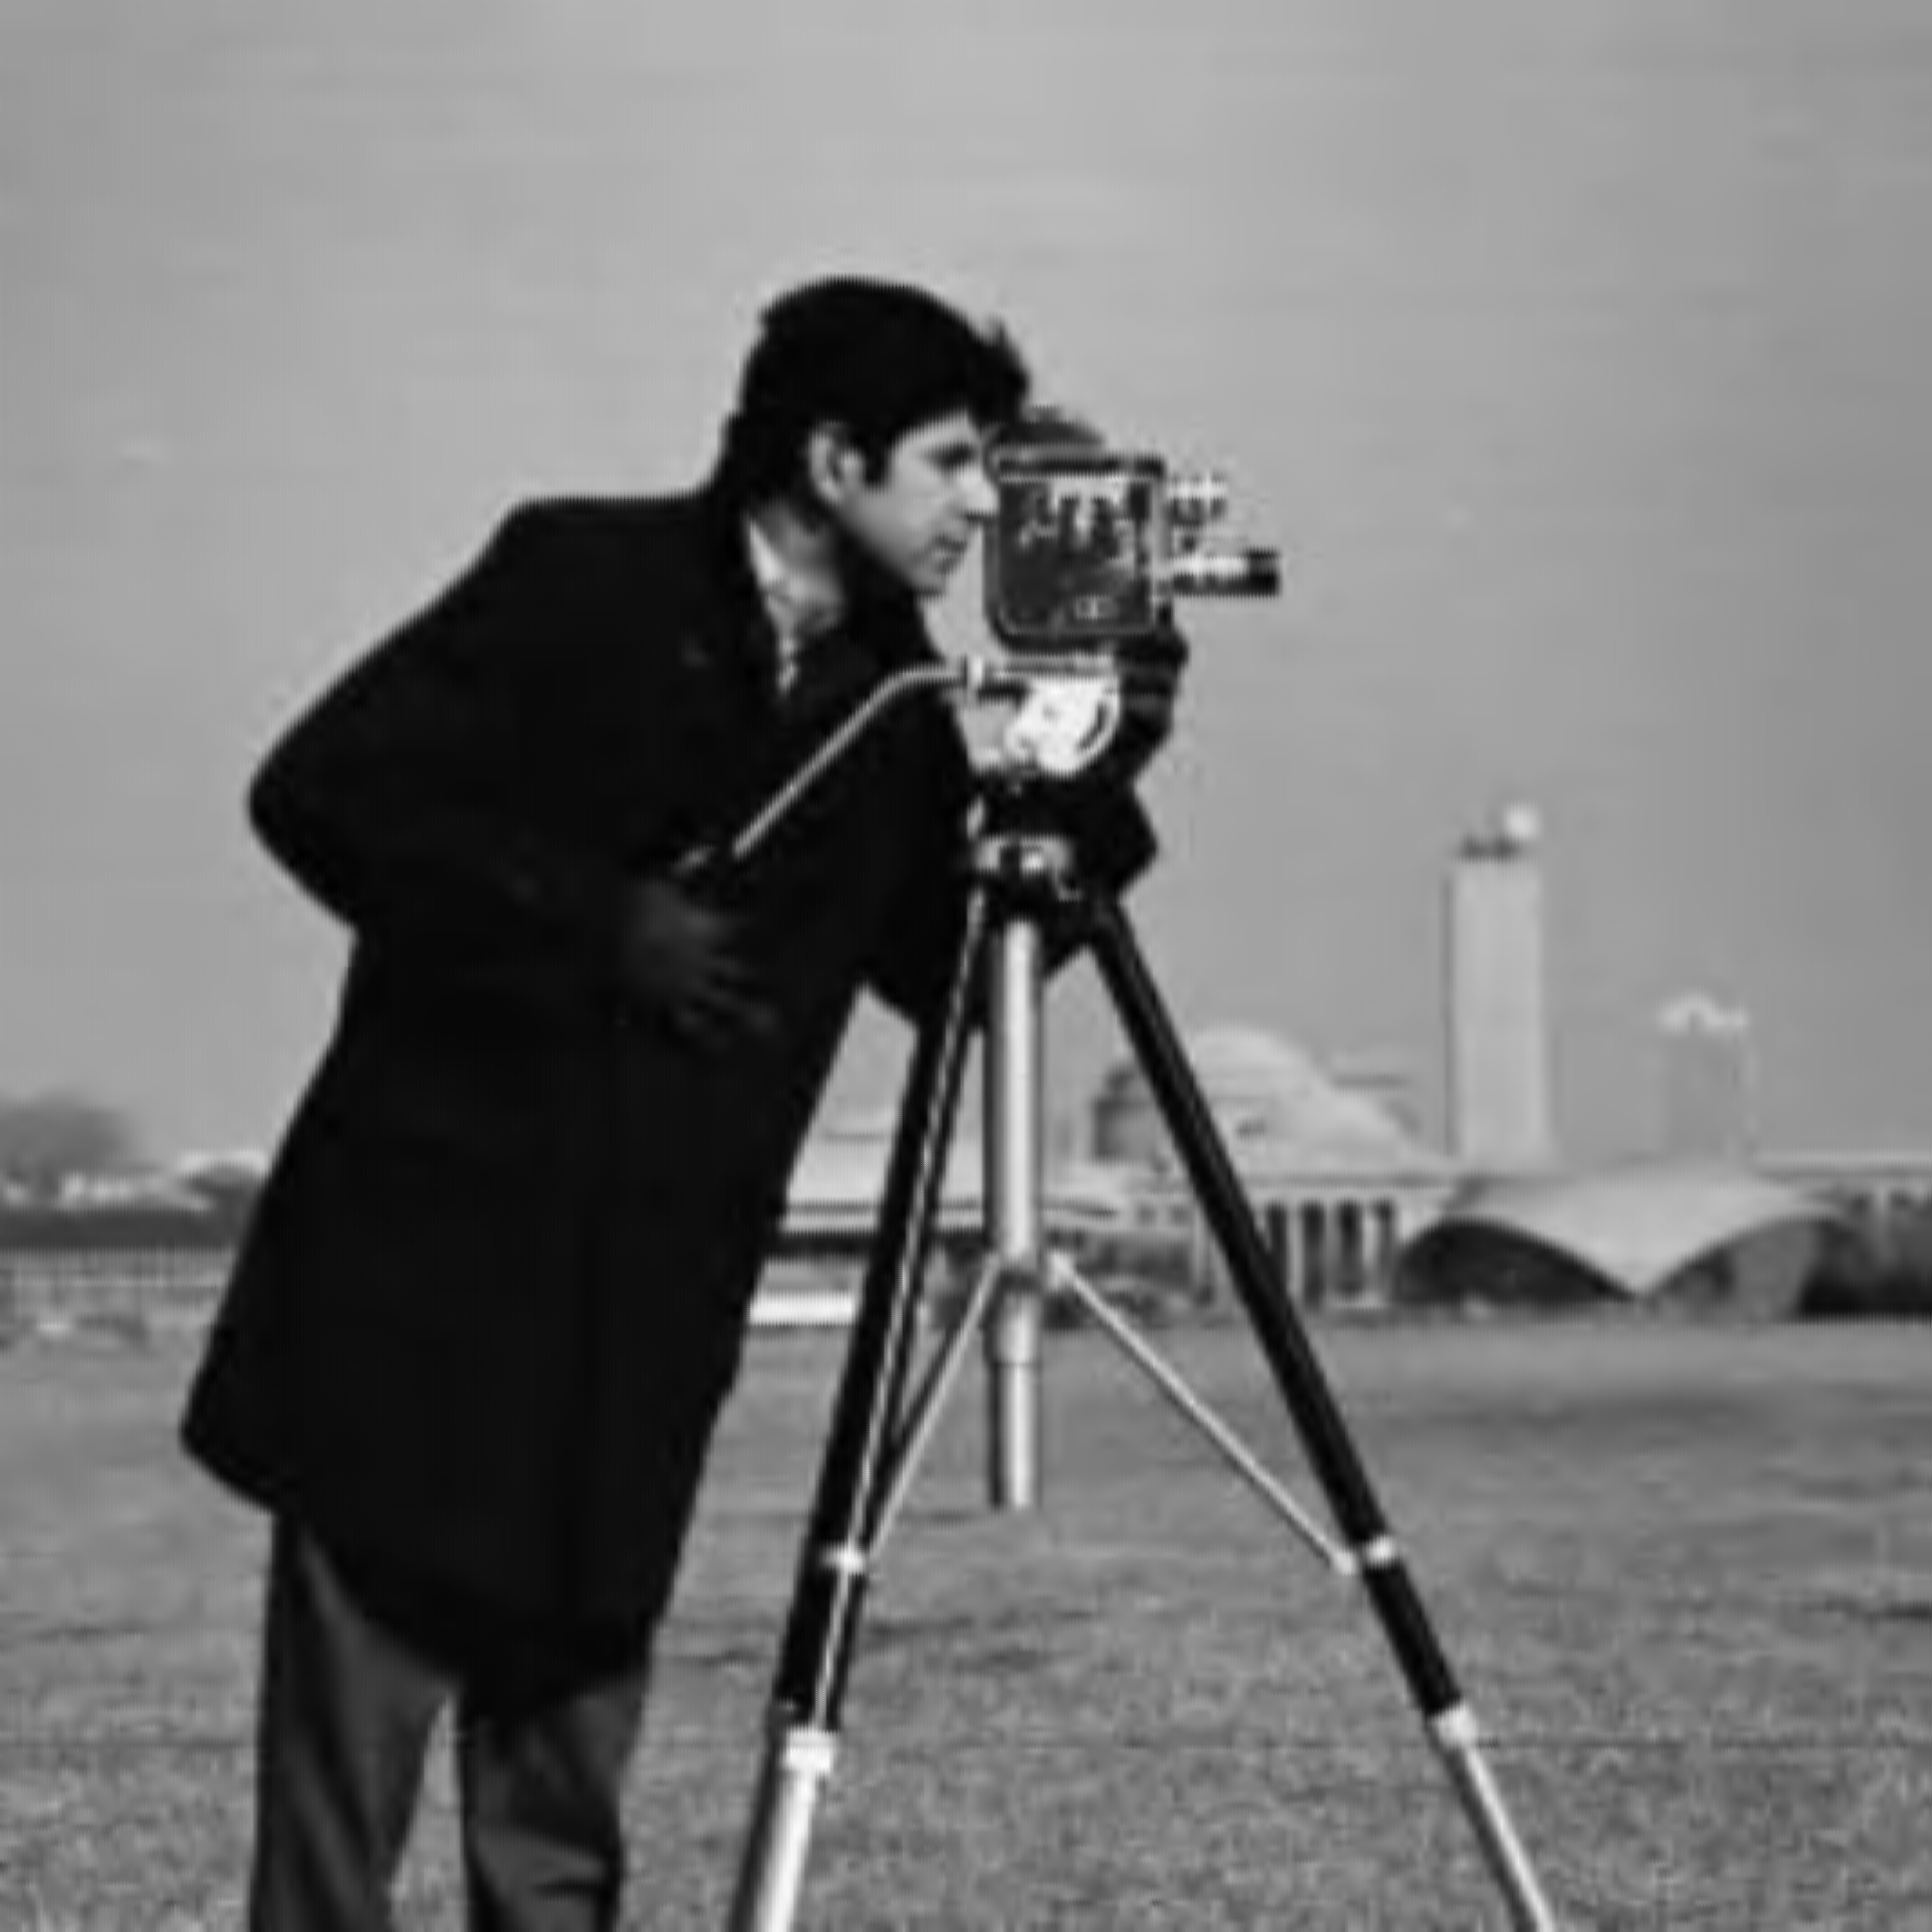
\includegraphics[width=8cm, height=8cm]{man-rastar-unification.png}
	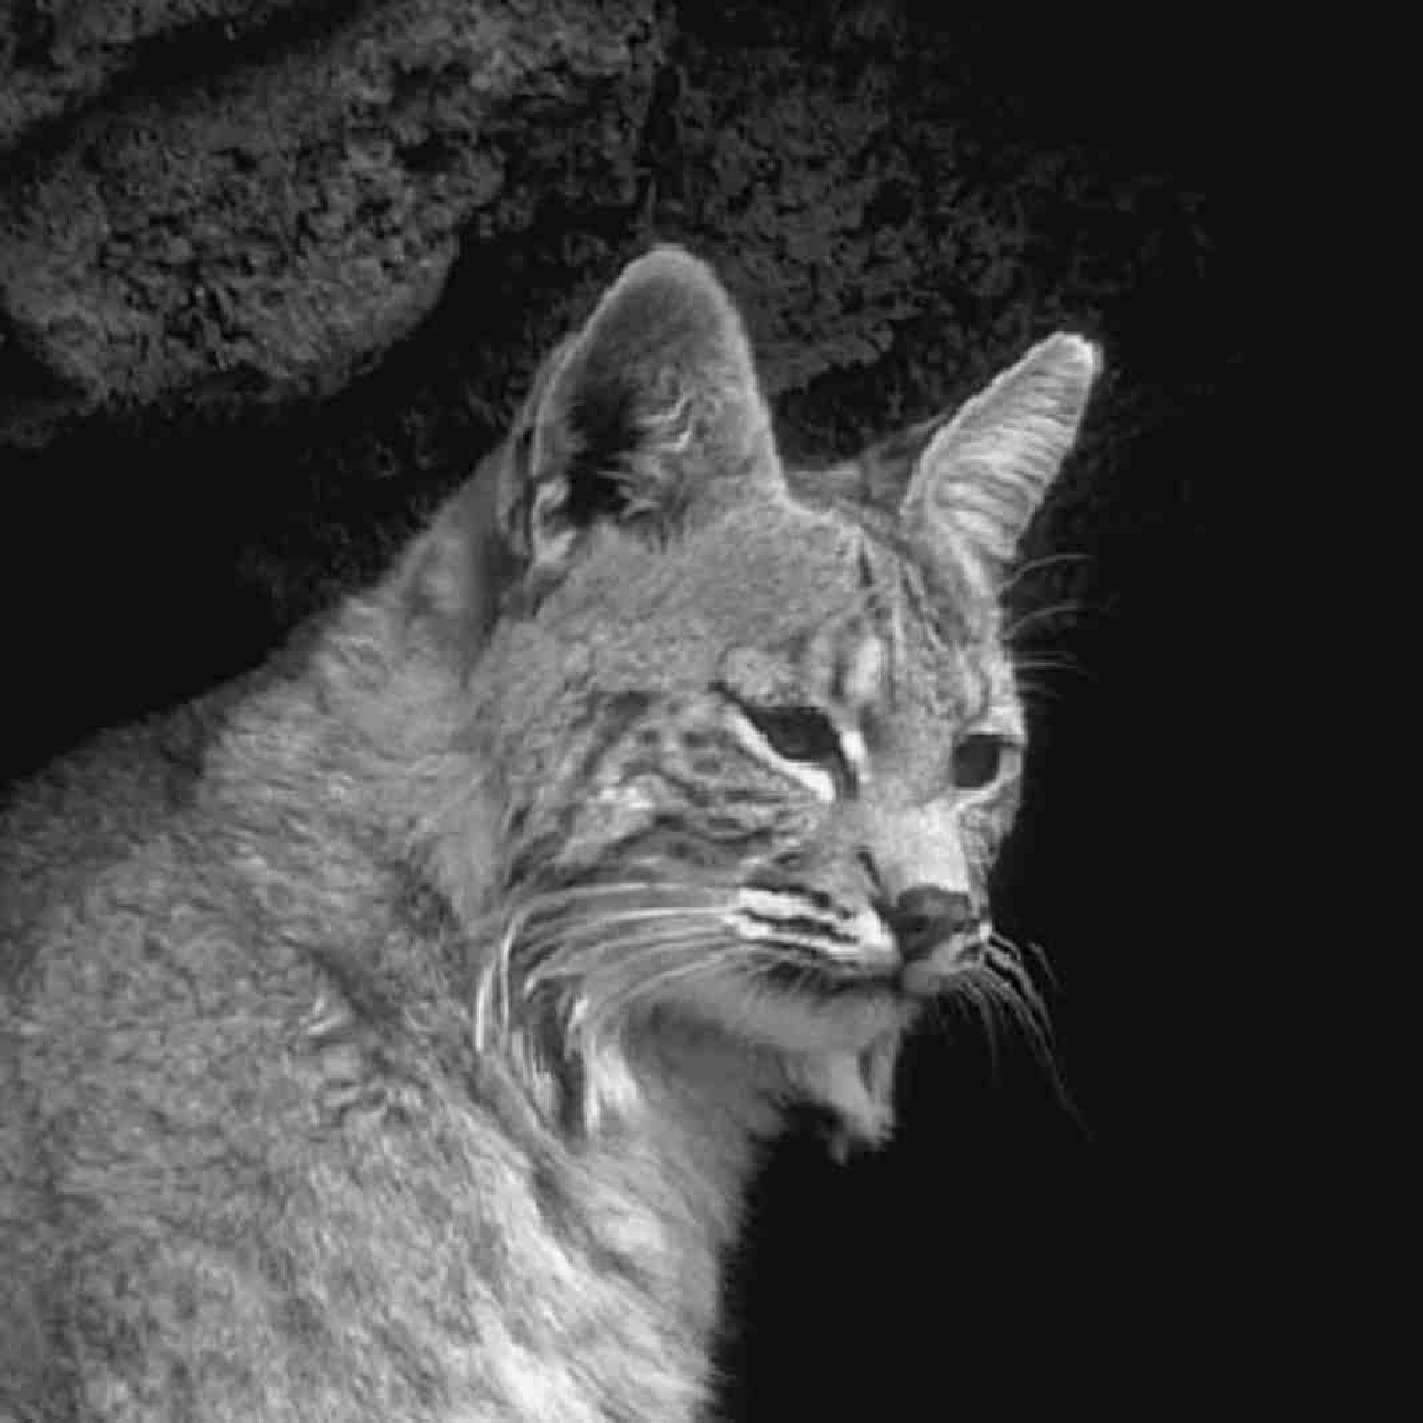
\includegraphics[width=8cm, height=8cm]{cat-unmodified.jpg}
\end{figure}
\subsection*{Kod źródłowy algorytmu}
\begin{python}
def rasterGray(self):
	print('raster gray unification start')
	self._scaleUpGray(self.firstDecoder, 'Resources/rgUnification_1.png')
	print('first image done')
	self._scaleUpGray(self.secondDecoder, 'Resources/rgUnification_2.png')
	print('second image done')
	print('raster gray unification done')

def _scaleUpGray(self, decoder, outputPath):
	width, height = decoder.width, decoder.height
	scaleFactoryW = float(self.maxWidth) / width
	scaleFactoryH = float(self.maxHeight) / height
	if width < self.maxWidth or height < self.maxHeight:
		pixelsBuffer = decoder.getPixels()
		result = numpy.zeros((self.maxHeight, self.maxWidth), numpy.uint8)
		# Fill values
		for h in range(height):
			for w in range(width):
				if w%2 == 0:
					result[int(scaleFactoryH * h), int(round(scaleFactoryW * w)) + 1] = pixelsBuffer[h, w]
				if w%2 == 1:
					result[int(round(scaleFactoryH * h)) + 1, int(scaleFactoryW * w)] = pixelsBuffer[h, w]
		# Interpolate
		self._interpolateGray(result)
		img = Image.fromarray(result, mode='L')
		img.save(outputPath)

def _interpolateGray(self, result):
	for h in range(self.maxHeight):
		for w in range(self.maxWidth):
			value = 0
			count = 0
			if result[h, w] == 0:
				for hOff in range(-1, 2):
					for wOff in range(-1, 2):
						hSafe = h if ((h + hOff) > (self.maxHeight - 2)) | ((h + hOff) < 0) else (h + hOff)
						wSafe = w if ((w + wOff) > (self.maxWidth - 2)) | ((w + wOff) < 0) else (w + wOff)
						if result[hSafe, wSafe] != 0:
							value += result[hSafe, wSafe]
							count += 1
				result[h, w] = value / count
\end{python}
\section{Ujednolicenie obrazów RGB geometryczne}
\subsection*{Algorytm}
\subsubsection*{Opis}
Algorytm geometrycznego ujednolicenia obrazów ma za zadanie sprowadzić oba obrazy do tej samej liczby pikseli w każdym wierszu i każdej kolumnie. 
Różnica pomiędzy tym przypadkiem a szarym sprawia, że ważne jest użycie odpowiednich struktur danych w taki sposób aby każdy z kanałów RGB był w stanie się pomieścić. Niewątpliwie ważne jest struktura danych uwzględniała kolejność w jakim kolory są przechowywane, inaczej może dojść do sytuacji w której nie dostaniemy oczekiwanego rezultatu. 
\subsubsection*{Kroki}
\begin{enumerate}
	\item Porównaj szerokości i wysokości obu obrazów i wybierz największe. 
	\item Jeśli pierwszy lub drugi obraz mają szerokość lub wysokość mniejszą od największej dostępnej to:
	\begin{enumerate}
		\item Utwórz czarne tło
		\item Przenieś z wyśrodkowaniem piksle na czarne tło z uwzględnieniem każdego z kanałów RGB
	\end{enumerate}
	\item Jeśli żaden z warunków jest niespełniony to nie rób nic
\end{enumerate}
\begin{figure}
	\caption{Przed uruchomieniem algorytmu (od lewej): obraz 1 (512x512, 300dpi), obraz 2 (1024x1024, 300dpi)}
	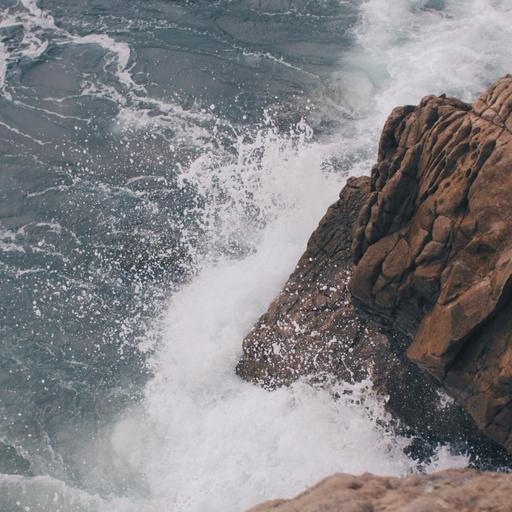
\includegraphics[width=8cm, height=8cm]{sea-unmodified.jpg}
	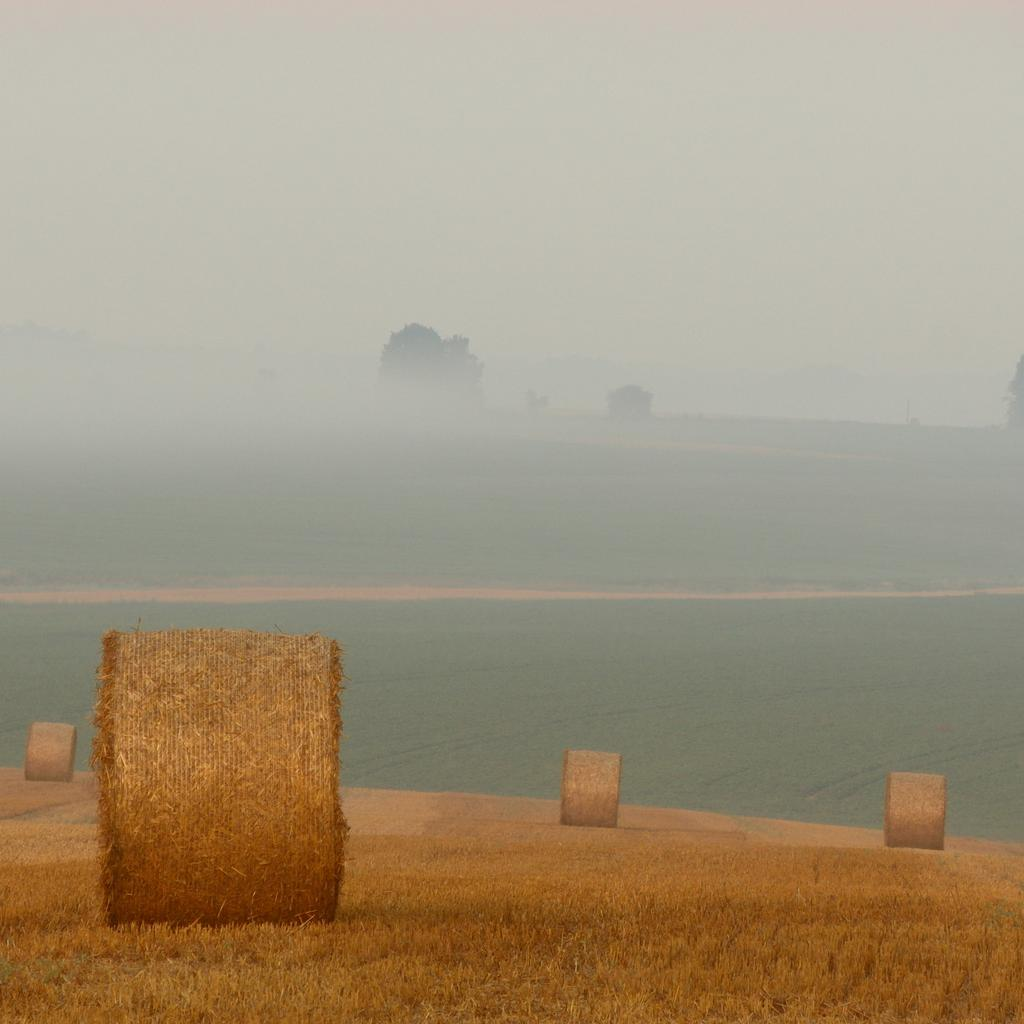
\includegraphics[width=8cm, height=8cm]{field-unmodified.jpg}
\end{figure}
\begin{figure}
	\caption{Po uruchomieniem algorytmu (od lewej): obraz 1 (1024x1024, 300dpi), obraz 2 (1024x1024, 300dpi)}
	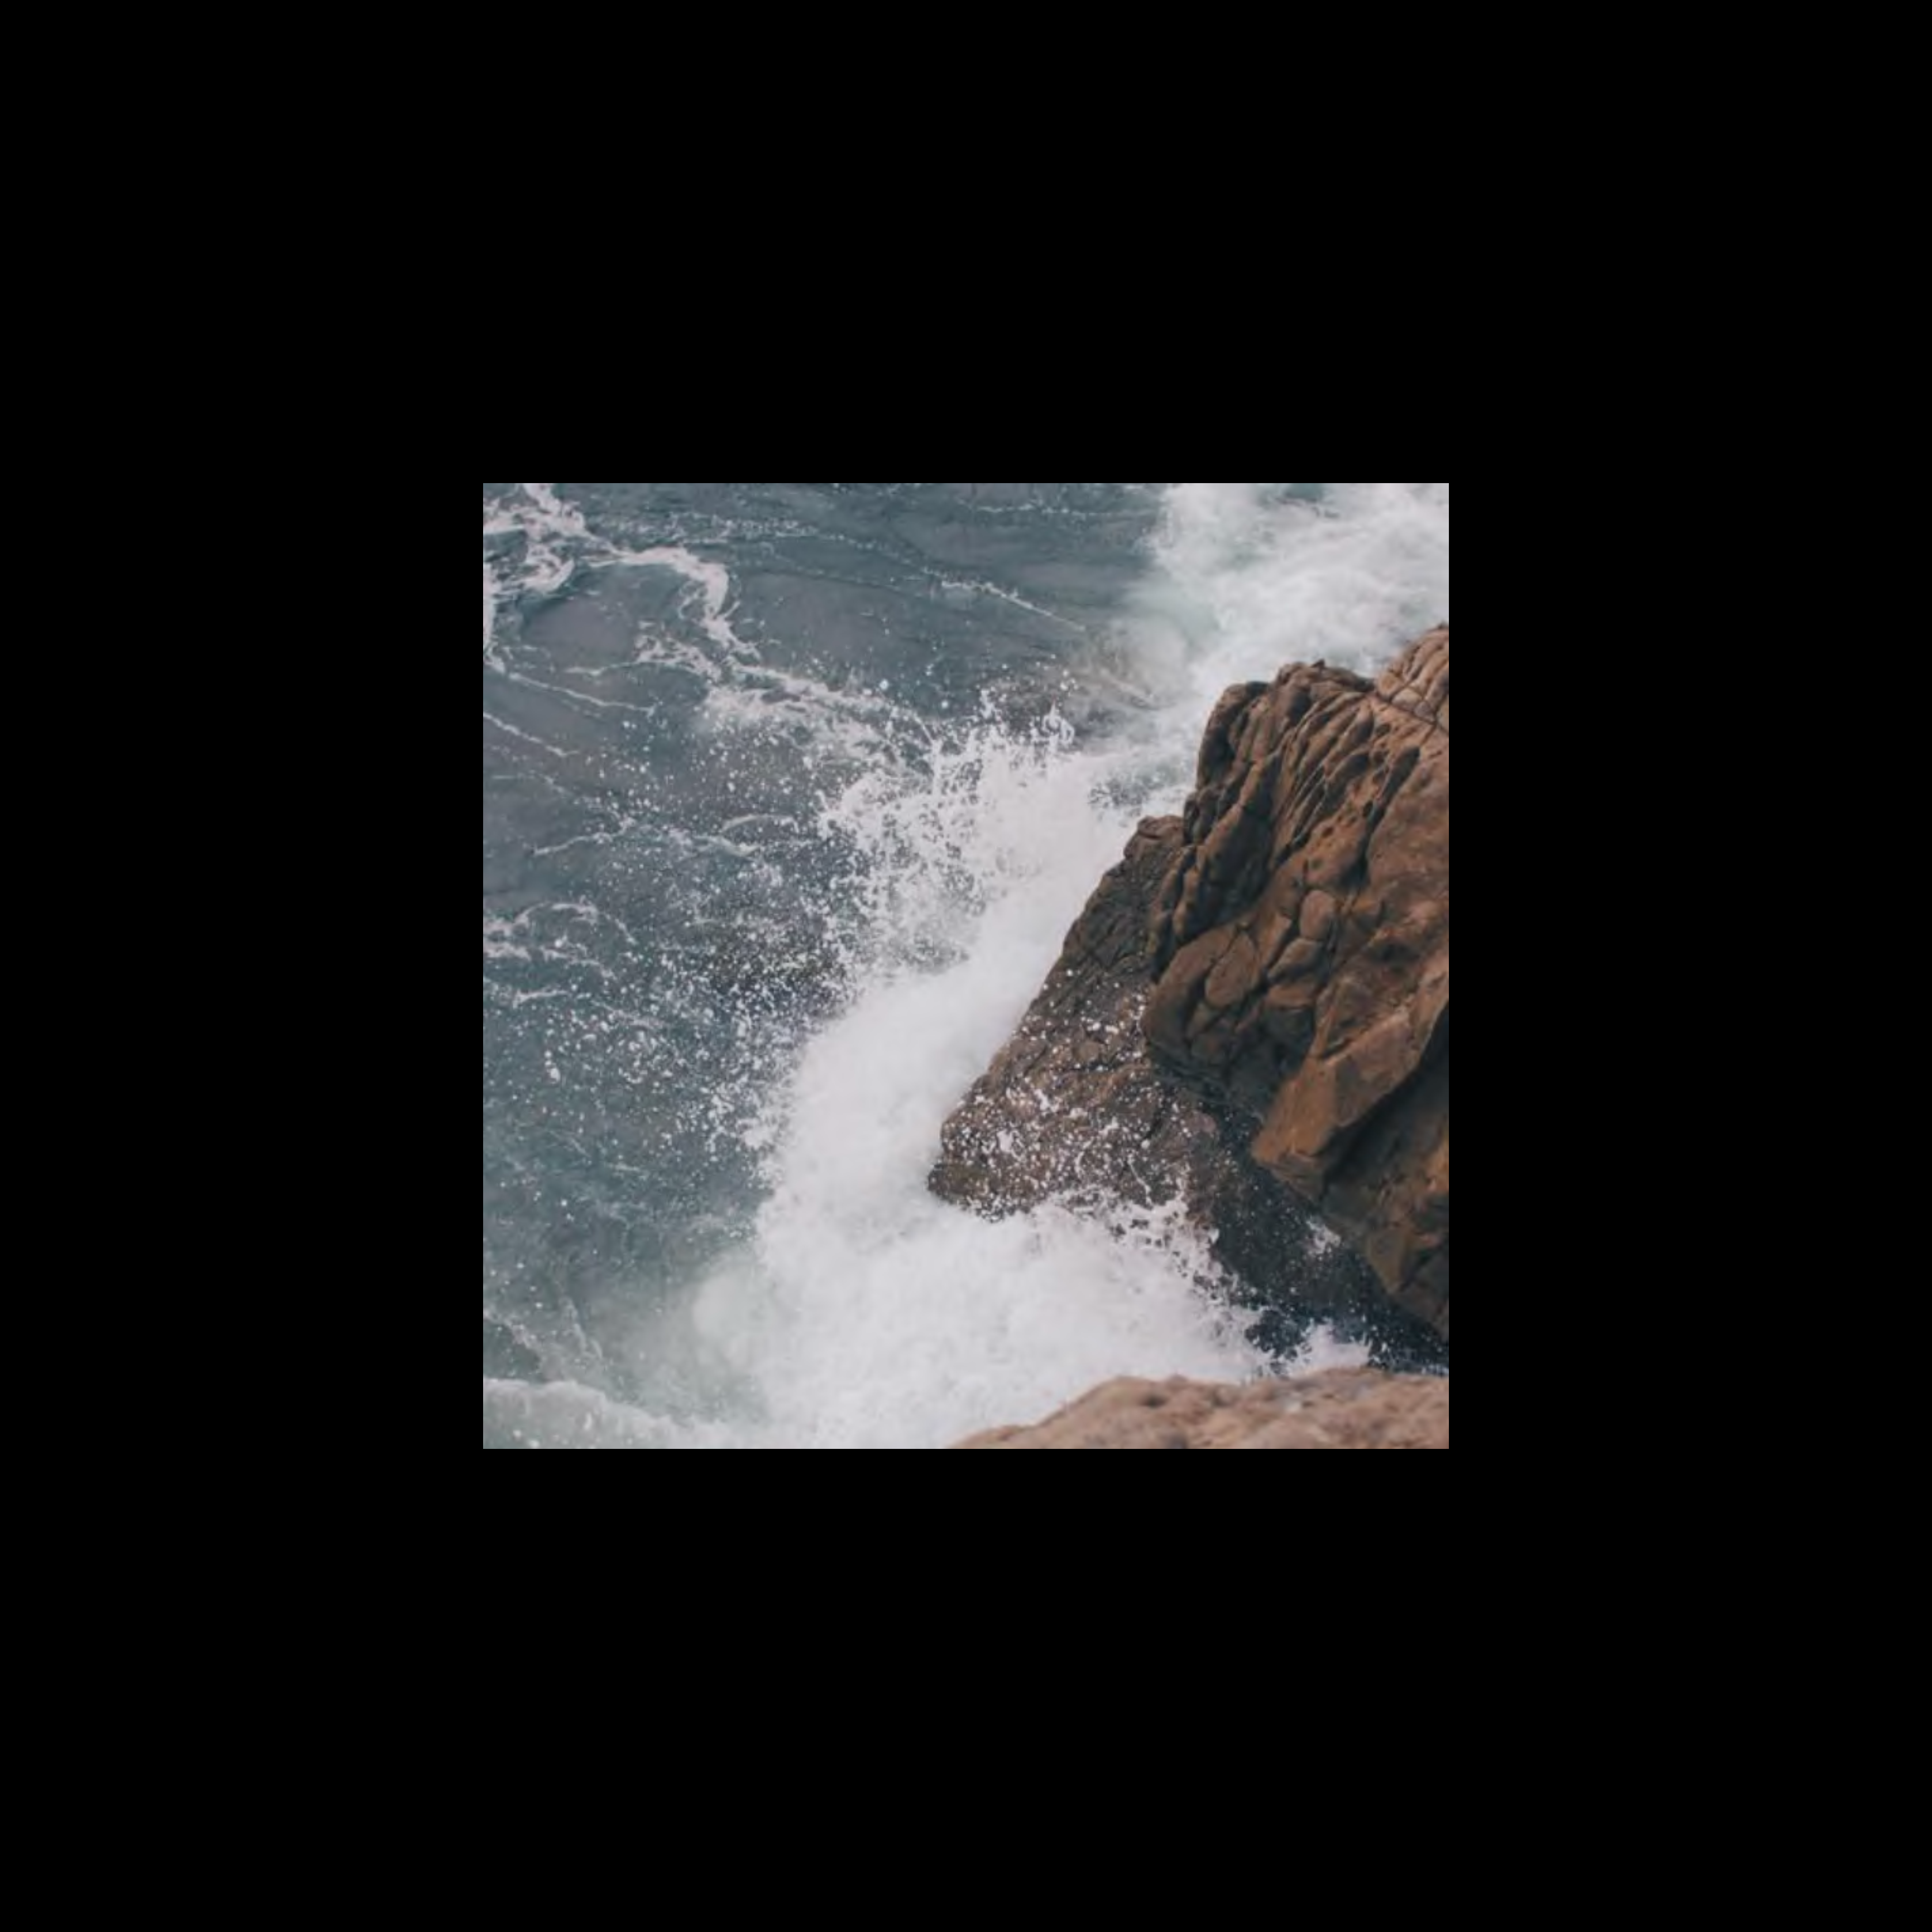
\includegraphics[width=8cm, height=8cm]{sea-geo-modified.png}
	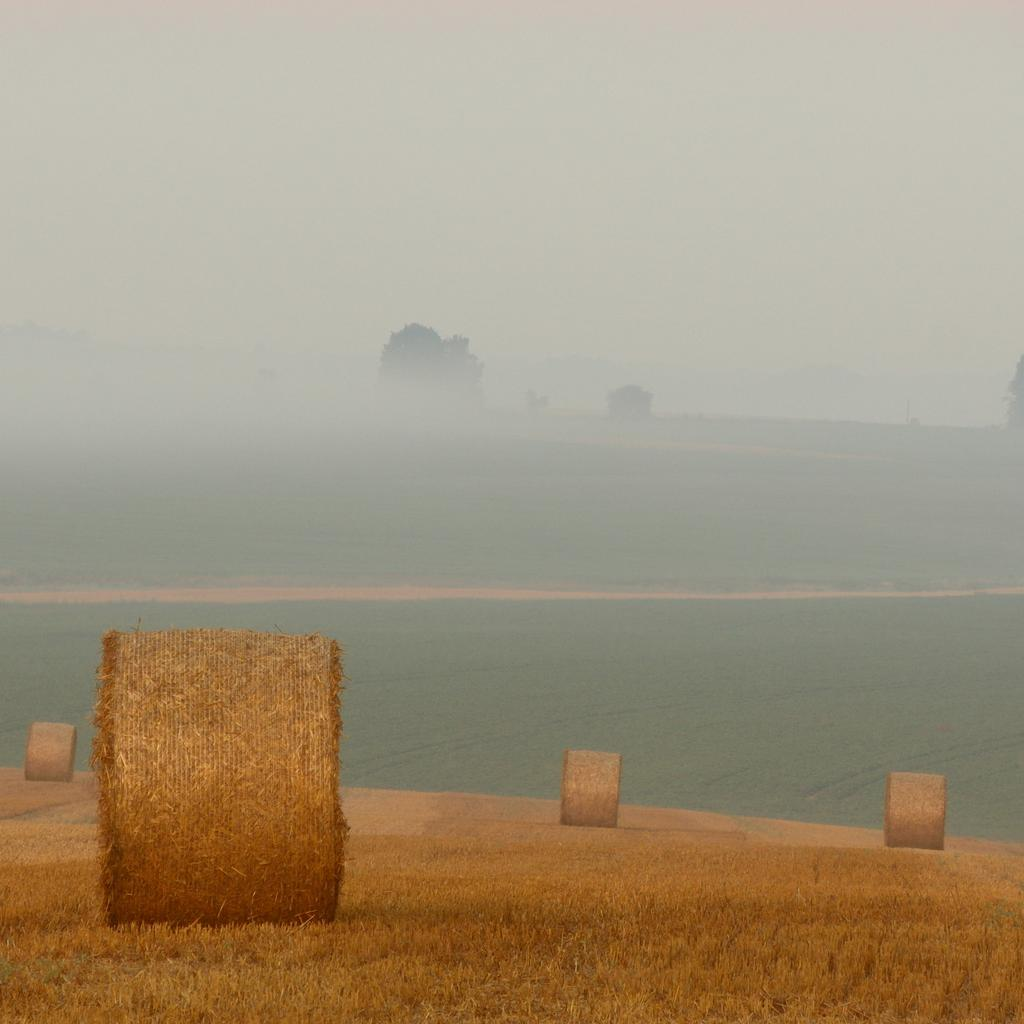
\includegraphics[width=8cm, height=8cm]{field-unmodified.jpg}
\end{figure}
\begin{figure}
	\caption{Przed uruchomieniem algorytmu (od lewej): obraz 3 (126x126, 300dpi), obraz 4 (256x256, 300dpi)}
	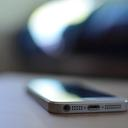
\includegraphics[width=8cm, height=8cm]{phone-unmodified.jpg}
	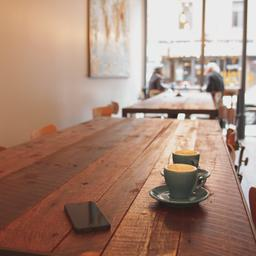
\includegraphics[width=8cm, height=8cm]{coffee-unmodified.jpg}
\end{figure}
\begin{figure}
	\caption{Po uruchomieniem algorytmu (od lewej): obraz 3 (126x126, 300dpi), obraz 4 (256x256, 300dpi)}
	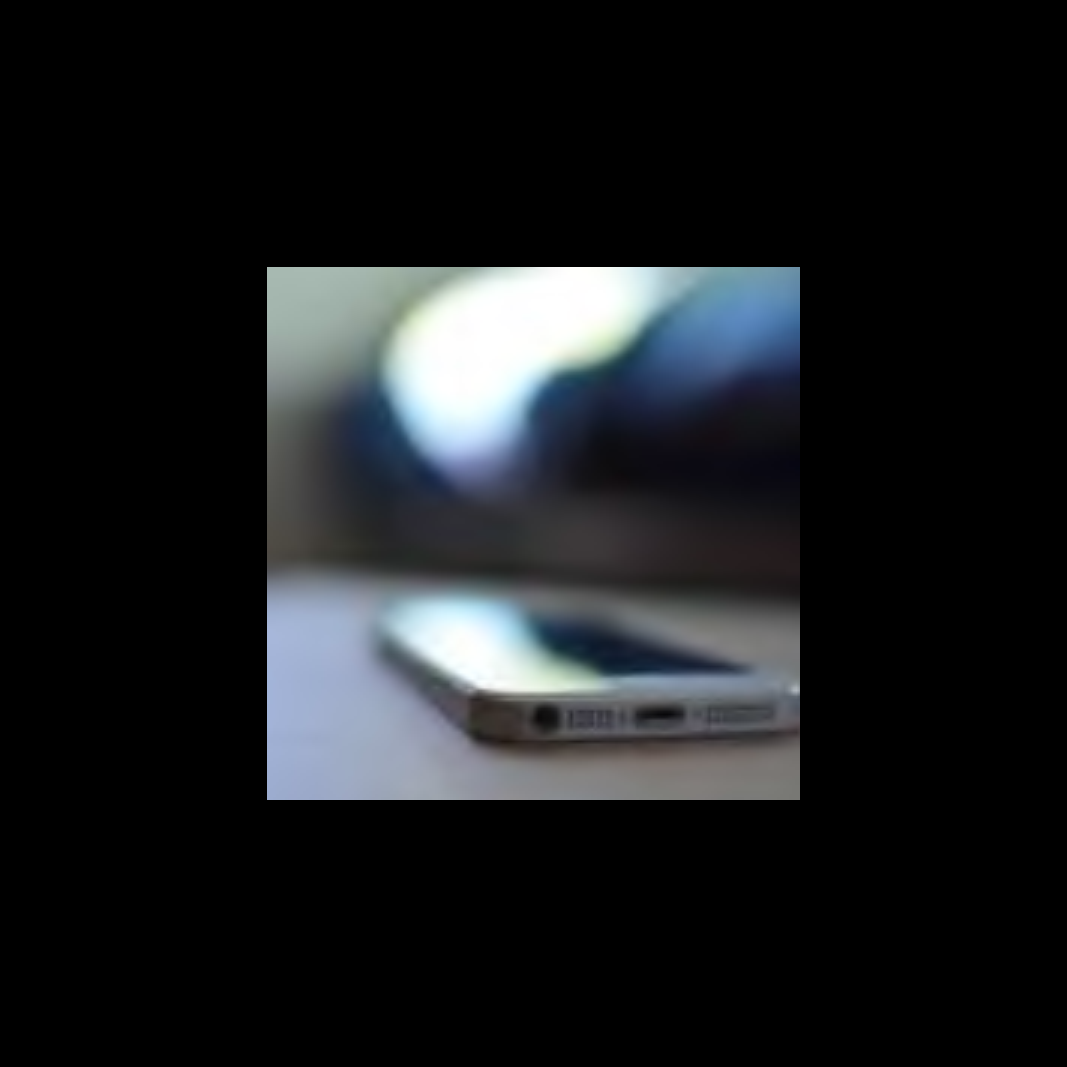
\includegraphics[width=8cm, height=8cm]{phone-geo-modified.png}
	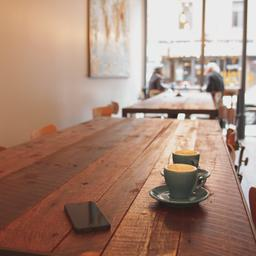
\includegraphics[width=8cm, height=8cm]{coffee-unmodified.jpg}
\end{figure}
\newpage
\subsection*{Kod źródłowy algorytmu}
\begin{python}
def geometricColor(self):
	print('geometric color unificaiton start')
	self.firstDecoder.setColor()
	width, height = self.firstDecoder.width, self.firstDecoder.height
	if width < self.maxWidth or height < self.maxHeight:
		result = self._paintInMiddleColor(self.firstDecoder)
		img = Image.fromarray(result, 'RGB')
		img.save('Resources/gcUnification_1.png')
		print('first image done')
	
	self.secondDecoder.setColor()
	width, height = self.secondDecoder.width, self.secondDecoder.height
	if width < self.maxWidth or height < self.maxHeight:
		result = self._paintInMiddleColor(self.secondDecoder)
		img = Image.fromarray(result, 'RGB')
		img.save('Resources/gcUnification_2.png')
		print('second image done')
	print('geometric color unification done')
	
def _paintInMiddleColor(self, decoder):
	# Create black background
	result = numpy.full((self.maxHeight, self.maxWidth, 3), 0, numpy.uint8)
	# Copy smaller image to bigger
	width, height = decoder.width, decoder.height
	startWidthIndex = int(round((self.maxWidth - width) / 2))
	startHeightIndex = int(round((self.maxHeight - height) / 2))
	pixelsBuffer = decoder.getPixels24Bits()
	for h in range (0, height):
		for w in range (0, width):
			result[h + startHeightIndex, w + startWidthIndex] = pixelsBuffer[h, w]
	return result
\end{python}
\section{Ujednolicenie obrazów RGB rozdzielczościowe}
\subsection*{Algorytm}
\subsubsection*{Opis}
Po użyciu ujednolicenia geometrycznego można użyć ujednolicenia rozdzielczościowego, które przeskaluje obraz z mniejszej postaci do większej dzięki czemu nie zostanie nam czarna ramka wokół obrazu. Wynikiem będzie większy obraz niż początkowo bez czarnego obwodu wokół. 
Mniejszy obraz można przeskalować do większych wymiarów przenosząc wszystkie piksele z uwzględnieniem luk pomiędzy nimi i następnie użycia interpolacji do zamazania tych luk. 
Interpolacja działa na zasadzie pobierania wartości z okolicznych pikseli i wyciągania z nich średniej, która posłuży jako baza koloru dla nowego piksela. 
\subsubsection*{Kroki}
\begin{enumerate}
	\item Ustalenie nowych wymiarów obrazu
	\item Obliczenie odległości pomiędzy pikselami (\textit{scaleFactoryH, scaleFactoryW})
	\item Naniesienie pikseli z mniejszego obrazu na większy z uwzględnieniem luk
	\item Interpolacja
\end{enumerate}
\begin{figure}
	\caption{Skutki braku interpolacji}
	\begin{center}
		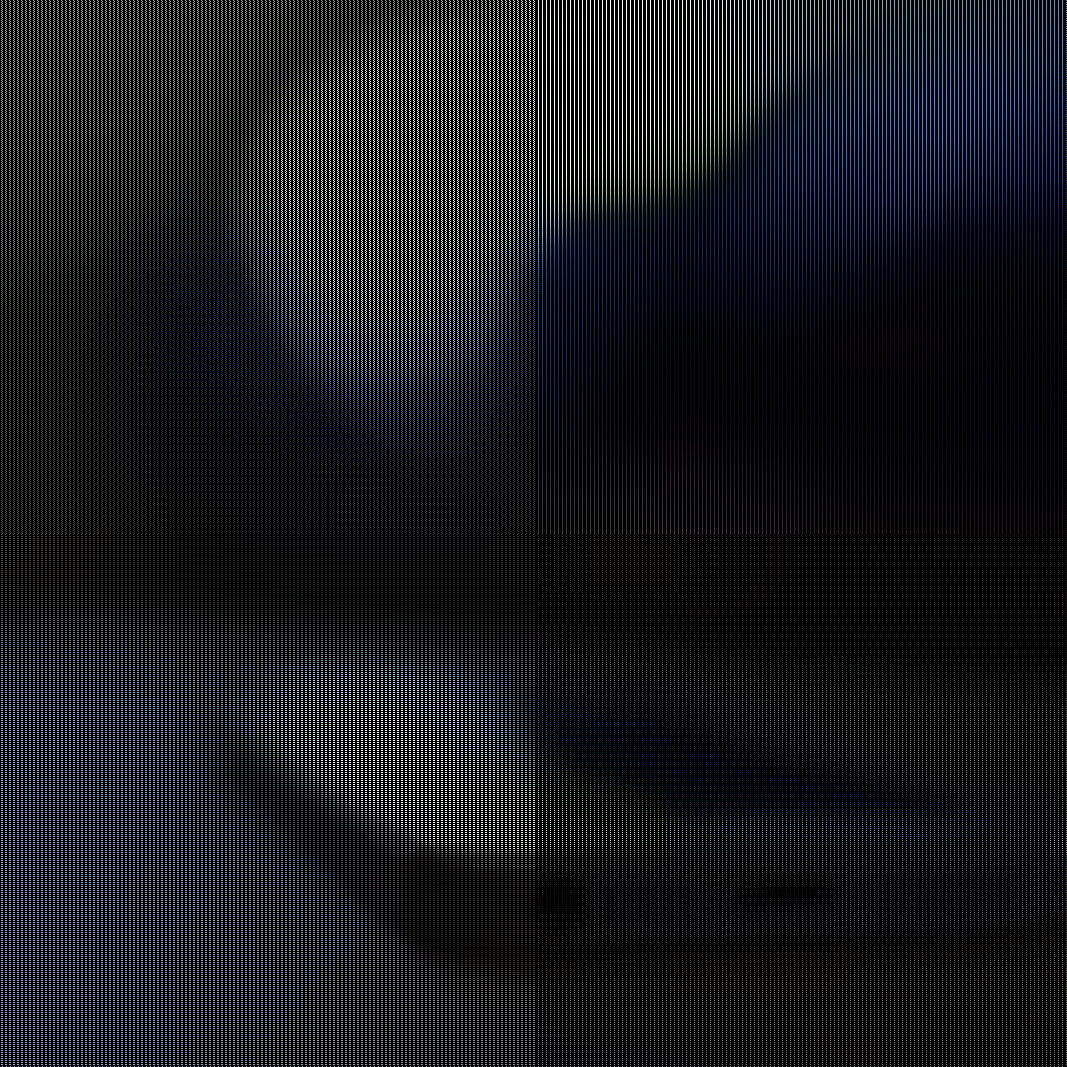
\includegraphics[width=8cm, height=8cm]{phone-without-interpolation.png}
	\end{center}
\end{figure}
\begin{figure}
	\caption{Przed uruchomieniem algorytmu (od lewej): obraz 1 (256x256, 300dpi), obraz 2 (256x256, 300dpi)}
	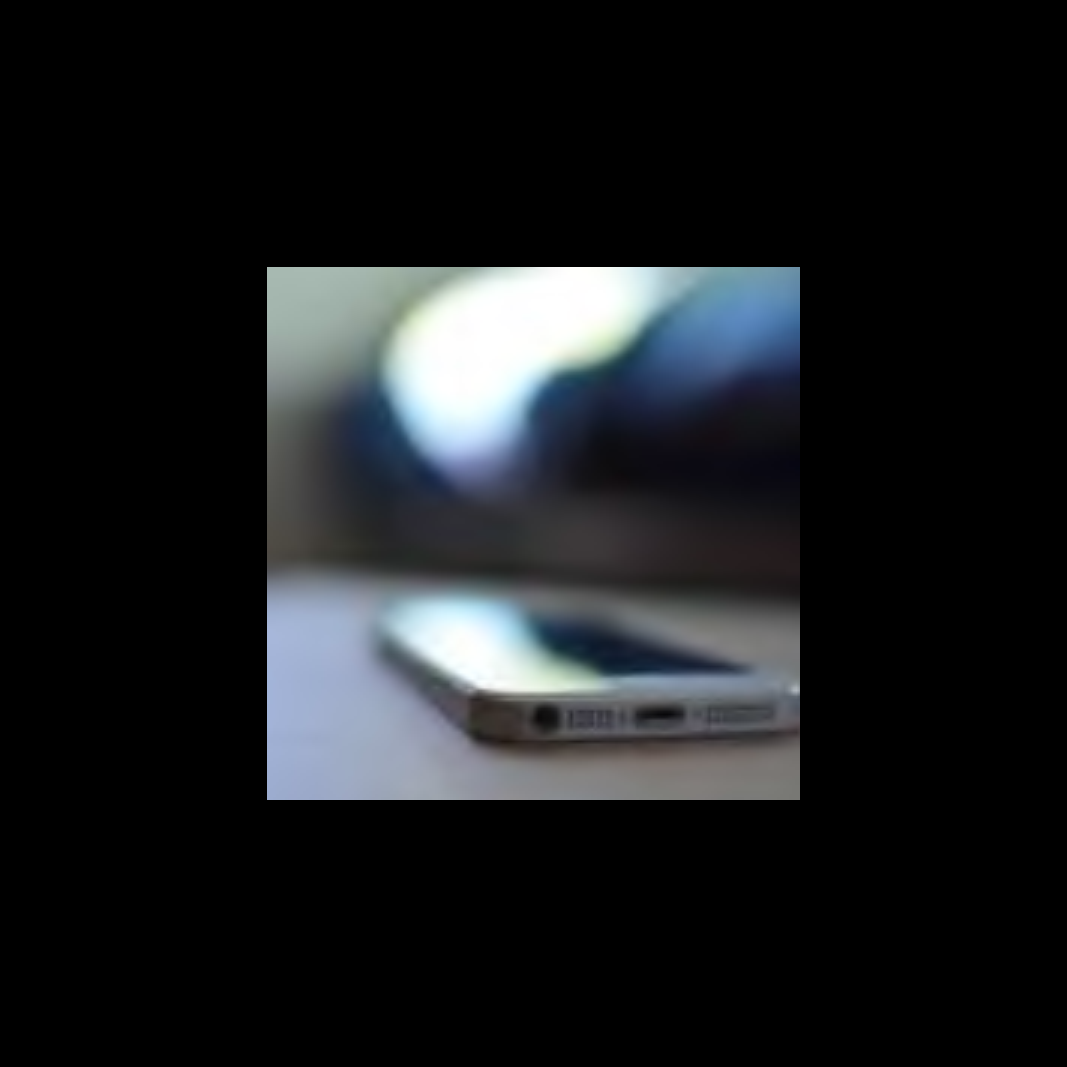
\includegraphics[width=8cm, height=8cm]{phone-geo-modified.png}
	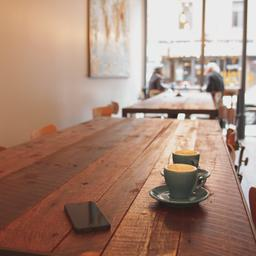
\includegraphics[width=8cm, height=8cm]{coffee-unmodified.jpg}
\end{figure}
\begin{figure}
	\caption{Po uruchomieniem algorytmu (od lewej): obraz 1 (256x256, 300dpi), obraz 2 (256x256, 300dpi)}
	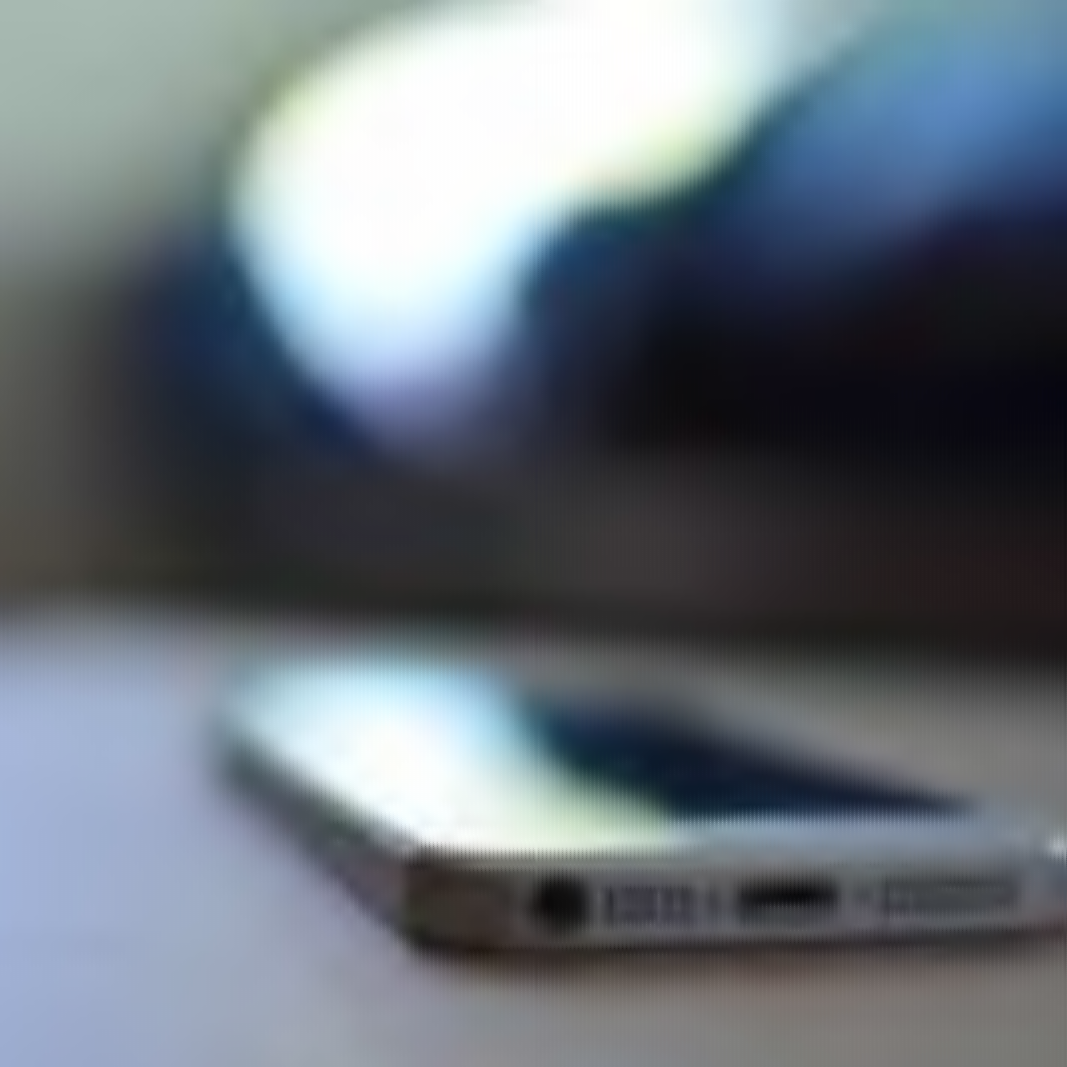
\includegraphics[width=8cm, height=8cm]{phone-rastar-unification.png}
	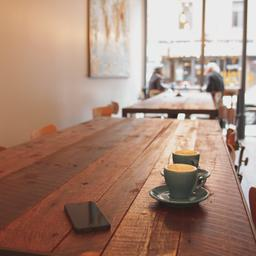
\includegraphics[width=8cm, height=8cm]{coffee-unmodified.jpg}
\end{figure}
\newpage
\subsection*{Kod źródłowy algorytmu}
\begin{python}
def rasterColor(self):
	print('rastar color unification start')
	self.firstDecoder.setColor()
	self._scaleUpColor(self.firstDecoder, 'Resources/rcUnification_1.png')
	print('first image done')
	self.secondDecoder.setColor()
	self._scaleUpColor(self.secondDecoder, 'Resources/rcUnification_2.png')
	print('second image done')
	print('rastar color unification done')

def _scaleUpColor(self, decoder, outputPath):
	width, height = decoder.width, decoder.height
	scaleFactoryW = float(self.maxWidth) / width
	scaleFactoryH = float(self.maxHeight) / height
	if width < self.maxWidth or height < self.maxHeight:
		pixelsBuffer = decoder.getPixels24Bits()
		result = numpy.full((self.maxHeight, self.maxWidth, 3), 1, numpy.uint8)
		# Fill values
		for h in range(height):
			for w in range(width):
				if w%2 == 0:
					result[int(scaleFactoryH * h), int(round(scaleFactoryW * w)) + 1] = pixelsBuffer[h, w]
				if w%2 == 1:
					result[int(round(scaleFactoryH * h)) + 1, int(scaleFactoryW * w)] = pixelsBuffer[h, w]
			# Interpolate
			self._interpolateColor(result)
			img = Image.fromarray(result, mode='RGB')
			img.save(outputPath)

def _interpolateColor(self, result):
	for h in range(self.maxHeight):
		for w in range(self.maxWidth):
			r, g, b = 0, 0, 0
			n = 0
			if (result[h, w][0] == 1) & (result[h, w][1] == 1) & (result[h, w][2] == 1):
				for hOff in range(-1, 2):
					for wOff in range(-1, 2):
						hSafe = h if ((h + hOff) > (self.maxHeight - 2)) | ((h + hOff) < 0) else (h + hOff)
						wSafe = w if ((w + wOff) > (self.maxWidth - 2)) | ((w + wOff) < 0) else (w + wOff)
						if (result[hSafe, wSafe][0] > 1) | (result[hSafe, wSafe][1] > 1) | (result[hSafe, wSafe][2] > 1):
							r += result[hSafe, wSafe][0]
							g += result[hSafe, wSafe][1]
							b += result[hSafe, wSafe][2]
							n += 1
				result[h, w] = (r/n, g/n, b/n)
\end{python}

\chapter{Operacje sumowania arytmetycznego obrazów szarych}
\section{Sumowanie (określonej) stałej z obrazem}
\section{Sumowanie dwóch obrazów}
\section{Mnożenie obrazu przez zadaną liczbę}
\section{Mnożenie obrazu przez inny obraz}
\section{Mieszanie obrazów z określonym współczynnikiem}
\section{Potęgowanie obrazu (z zadaną potęgą)}
\section{Dzielenie obrazu przez (zadaną) liczbę}
\section{Dzielenie obrazu przez przez inny obraz}
\section{Pierwiastkowanie obrazu}
\section{Logarytmowanie obrazu}

\chapter{Operacje sumowania arytmetycznego obrazów barwowych}
\section{Sumowanie (określonej) stałej z obrazem}
\section{Sumowanie dwóch obrazów}
\section{Mnożenie obrazu przez zadaną liczbę}
\section{Mnożenie obrazu przez inny obraz}
\section{Mieszanie obrazów z określonym współczynnikiem}
\section{Potęgowanie obrazu (z zadaną potęgą)}
\section{Dzielenie obrazu przez (zadaną) liczbę}
\section{Dzielenie obrazu przez przez inny obraz}
\section{Pierwiastkowanie obrazu}
\section{Logarytmowanie obrazu}

\chapter{Operacje geometryczne na obrazie}
Operacje geometryczne przekształcają położenie pikseli \textit{(x1, y1)} w obrazie wejściowym do nowej lokacji \textit{(x2, y2)} w obrazie wynikowym. Dzięki temu możemy dopasować obraz do odpowiedniego układu współrzędnych lub użyć tych operacji do eliminacji geometrycznych zakłóceń obrazu (dystorsji). 
\section{Przemieszczenie obrazu o zadany wektor}
\subsection*{Opis}
Operacja translacji wykonuje transformację geometryczną polegającą na przeniesieniu każdego z punktów obrazu wejściowego w nowe miejsce na obrazie wynikowym. Pod wpływem translacji element obrazu zlokalizowany na \textit{(x1, y1)} zostanie przesunięty na nową pozycję \textit{(x2, y2)}. Różnicą pomiędzy \textit{(x1, y1)} i \textit{(x2, y2)} jest wektor \textit{(bx, by)}, który jest określony przez użytkownika. 
\newline
Operacja przemieszczenia przybiera postać: 
\begin{gather}
	x_2 = x_1 + b_x \\
	y_2 = y_1 + b_y
\end{gather}
\begin{figure}[H]
	\caption{Przed uruchomieniem algorytmu (lewy obraz), po przesunięciu o wektor [100, 100] (prawy obraz)}
	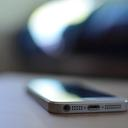
\includegraphics[width=8cm, height=8cm]{phone-unmodified.jpg}
	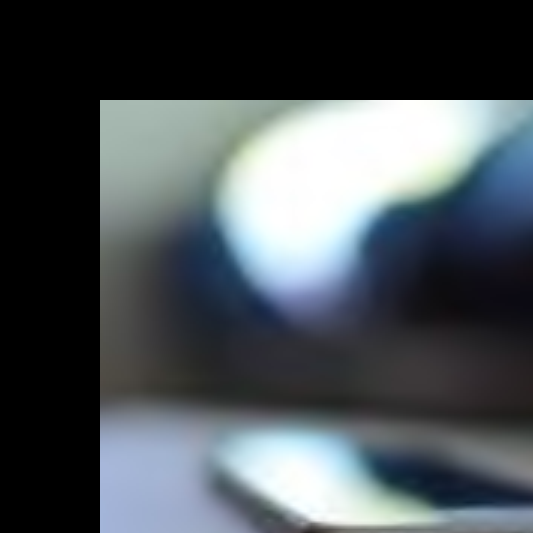
\includegraphics[width=8cm, height=8cm]{phone-translate.png}
\end{figure}
\begin{figure}[H]
	\caption{Przed uruchomieniem algorytmu (lewy obraz), po przesunięciu o wektor [100, -100] (prawy obraz)}
	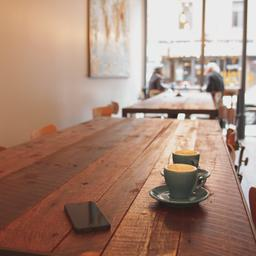
\includegraphics[width=8cm, height=8cm]{coffee-unmodified.jpg}
	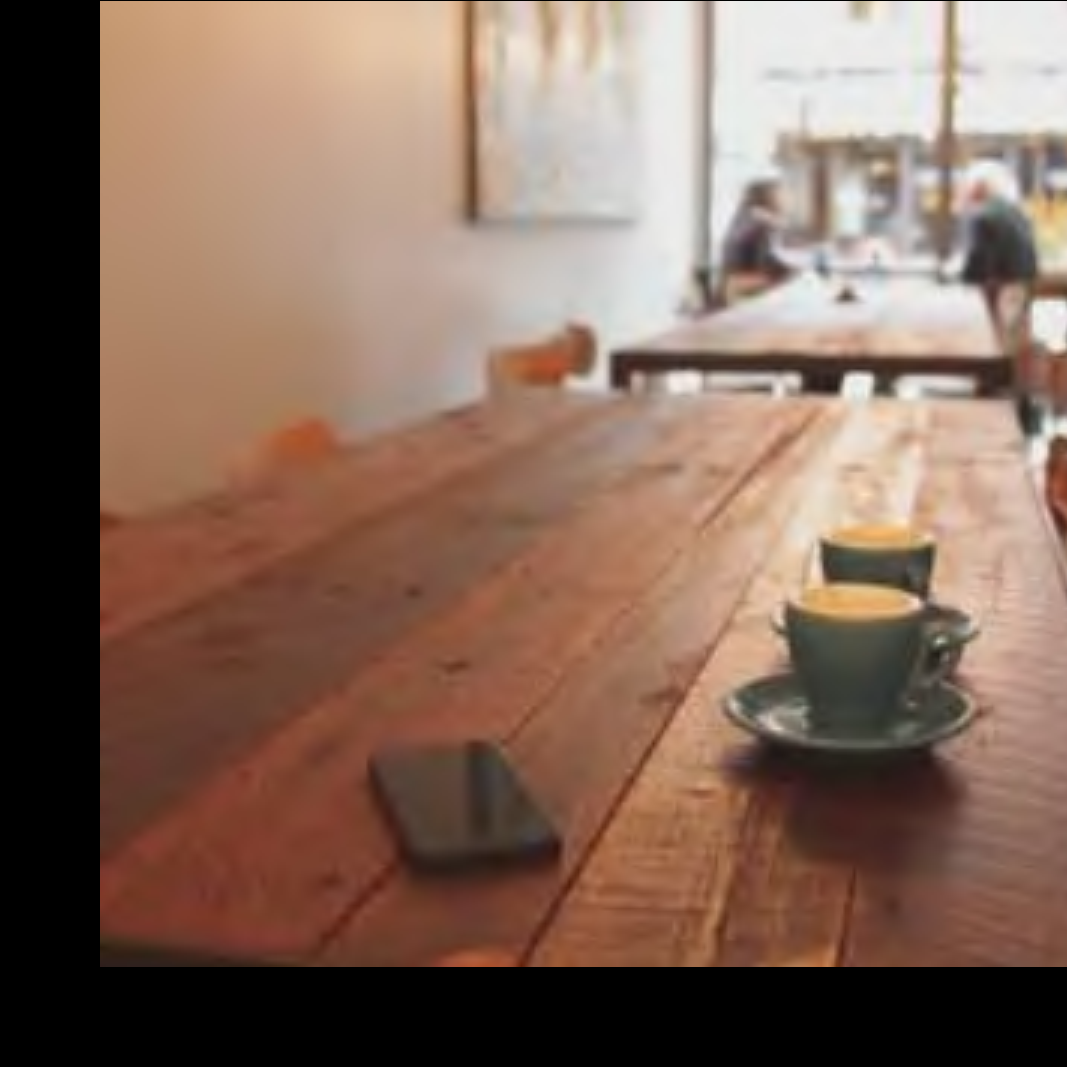
\includegraphics[width=8cm, height=8cm]{coffee-translate.png}
\end{figure}
\subsection*{Kod źródłowy algorytmu}
\begin{python}
def translate(self, deltaX = 0, deltaY = 0):
	print('translation start')
	height, width = self.decoder.height, self.decoder.width
	image = self.decoder.getPixels24Bits()
	result = numpy.zeros((height, width, 3), numpy.uint8)
	
	for y in range(height):
		for x in range(width):  
			if 0 < y + deltaY < height and 0 < x + deltaX < width:
				result[y + deltaY][x + deltaX] = image[y][x]
	
	img = Image.fromarray(result, mode='RGB')
	img.save('Resources/tGeometric.png')
print('translation done')
\end{python}
\section{Jednorodne skalowanie obrazu}
\subsection*{Opis}
Skalowanie jednorodne obrazu składa się na pomnożenie współrzędnych każdego piksela przez określoną wartość. 
\begin{gather}
x_2 = S_x * x_1 \\
y_2 = S_y * y_1
\end{gather}
Przy czym skalowanie jednorodne oznacza, że po zmianie wartości współrzędnych nasz obraz zachowa dawne proporcje. Czyli: 
\begin{gather}
S_x = S_y
\end{gather}
\begin{figure}[H]
	\caption{Przed uruchomieniem algorytmu (lewy obraz), po skalowaniu jednorodnym o współczynnik 2 (prawy obraz)}
	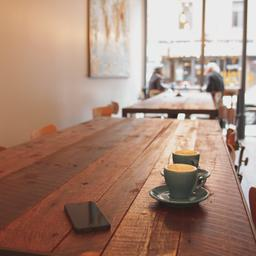
\includegraphics[width=4cm, height=4cm]{coffee-unmodified.jpg}
	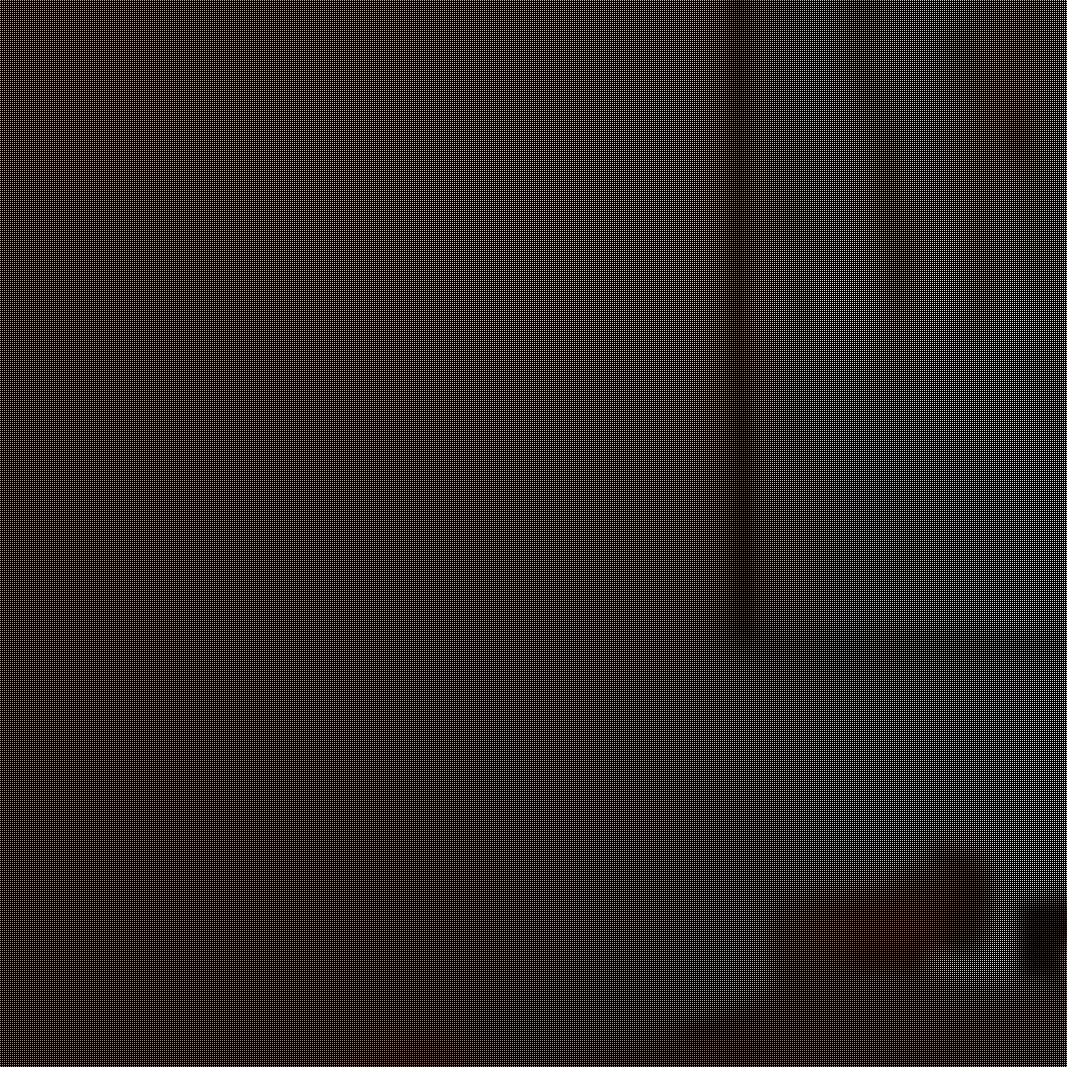
\includegraphics[width=4cm, height=4cm]{coffee-hscaling-without-interpolation.png}
	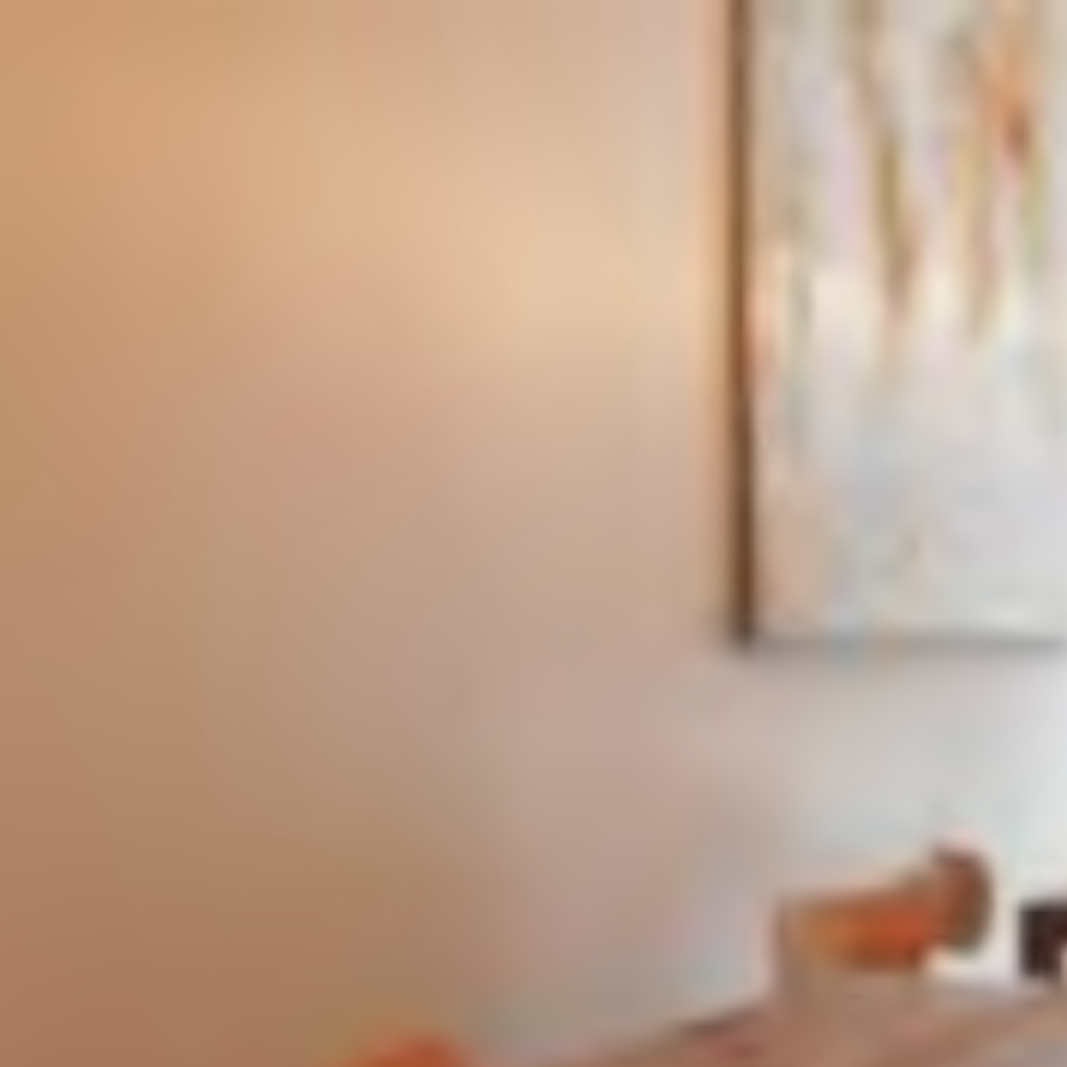
\includegraphics[width=4cm, height=4cm]{coffee-hscaling.png}
\end{figure}
\subsection*{Kod źródłowy algorytmu}
\begin{python}
def homogeneousScaling(self, scale = 1.0):
	print('homogeneous scaling start')
	image = self.decoder.getPixels24Bits()
	
	print('scaling')
	result = self._scaleXY(image, scale)
	print('interpolation')
	self._interpolateColor(result)
	
	img = Image.fromarray(result, mode='RGB')
	img.save('Resources/hsGeometric.png')
	print('homogeneous scaling done')

def _scaleXY(self, matrix, scale):
	height, width = self.decoder.height, self.decoder.width
	result = numpy.full((height, width, 3), 1, numpy.uint8)
	for y in range(height):
		for x in range(width):  
			if scale * y < height and scale * x < width:
				result[int(scale * y)][int(scale * x)] = matrix[y][x]
	return result

def _interpolateColor(self, result):
	height, width = self.decoder.height, self.decoder.width
	for h in range(height):
		for w in range(width):
			r, g, b = 0, 0, 0
			n = 0
			if (result[h, w][0] == 1) & (result[h, w][1] == 1) & (result[h, w][2] == 1):
				for hOff in range(-1, 2):
					for wOff in range(-1, 2):
						hSafe = h if ((h + hOff) > (height - 2)) | ((h + hOff) < 0) else (h + hOff)
						wSafe = w if ((w + wOff) > (width - 2)) | ((w + wOff) < 0) else (w + wOff)
						if (result[hSafe, wSafe][0] > 1) | (result[hSafe, wSafe][1] > 1) | (result[hSafe, wSafe][2] > 1):
							r += result[hSafe, wSafe][0]
							g += result[hSafe, wSafe][1]
							b += result[hSafe, wSafe][2]
							n += 1
				result[h, w] = (r/n, g/n, b/n)
\end{python}
\section{Niejednorodne skalowanie obrazu}
\subsection*{Opis}
Skalowanie niejednorodne obrazu składa się na pomnożenie współrzędnych każdego piksela przez określoną wartość. 
\begin{gather}
x_2 = S_x * x_1 \\
y_2 = S_y * y_1
\end{gather}
Przy czym skalowanie niejednorodne oznacza, że po zmianie wartości współrzędnych nasz obraz będzie miał zachwiane proporcje. Czyli: 
\begin{gather}
S_x \neq S_y
\end{gather}
\begin{figure}[H]
	\caption{Przed uruchomieniem algorytmu (lewy obraz), po skalowaniu jednorodnym o współczynnik x = 2.0, y = 1.0 (prawy obraz)}
	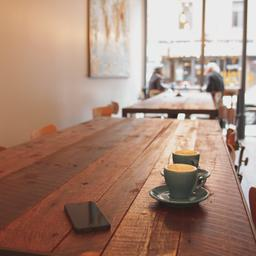
\includegraphics[width=4cm, height=4cm]{coffee-unmodified.jpg}
	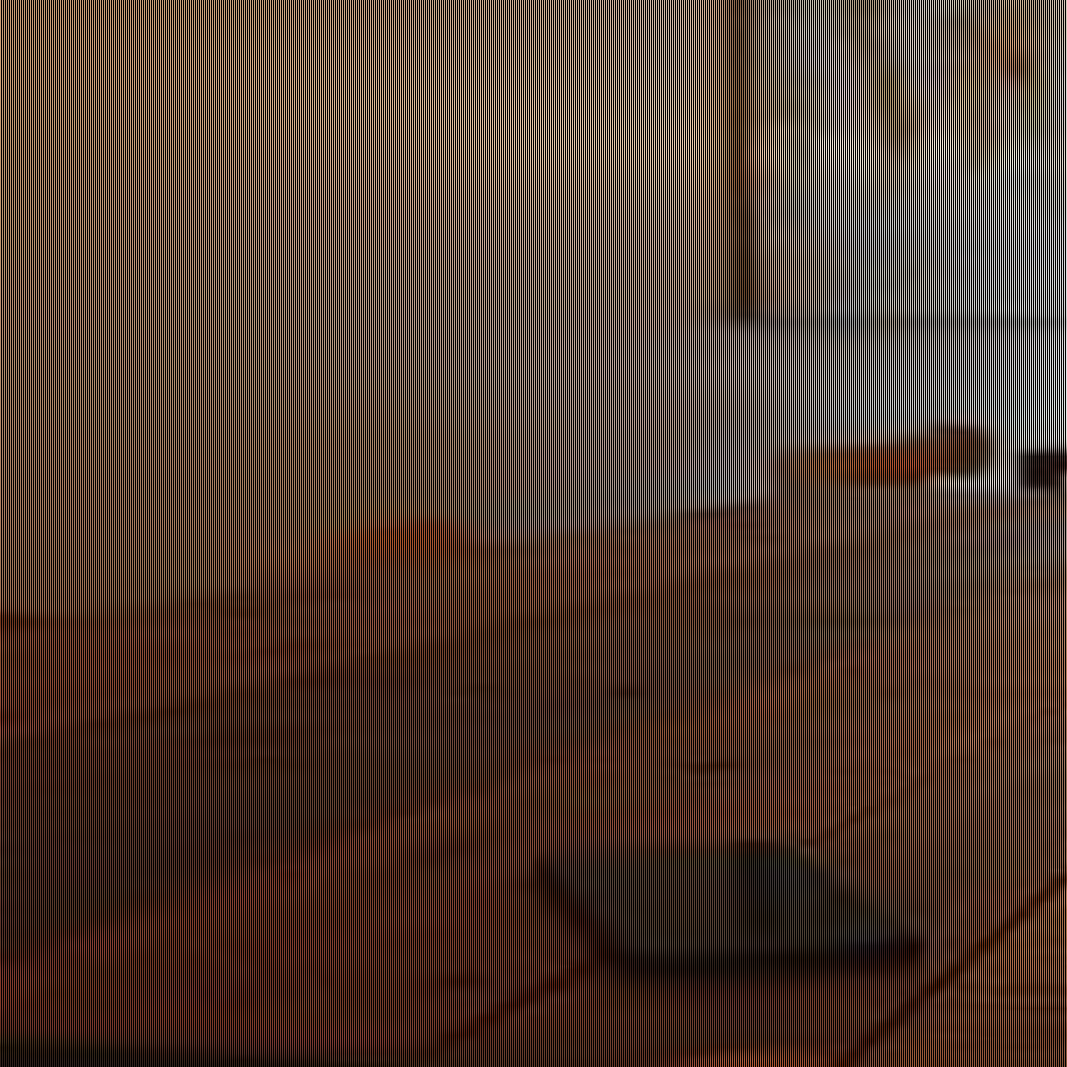
\includegraphics[width=4cm, height=4cm]{coffee-nonuniform-scaling-without-interpolation.png}
	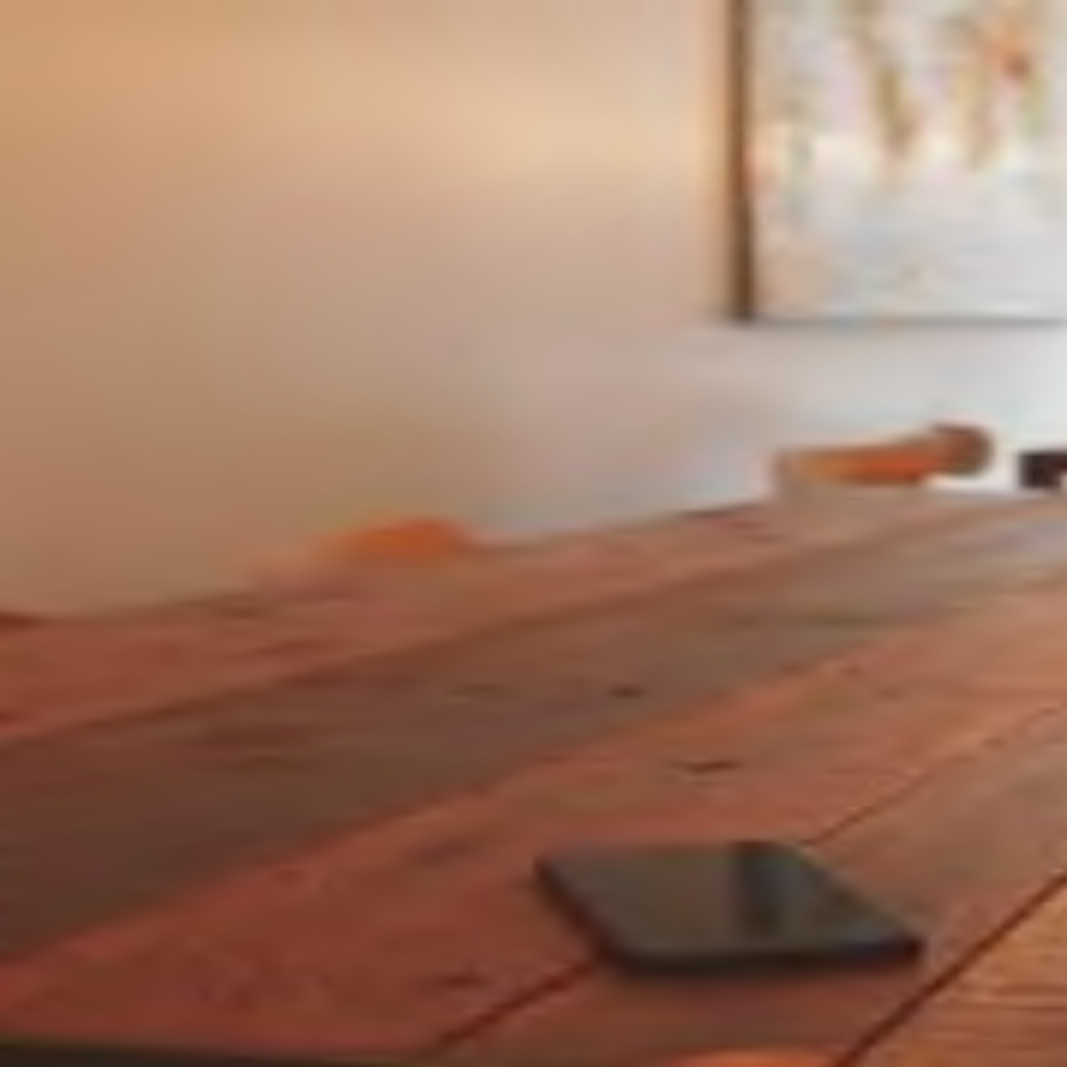
\includegraphics[width=4cm, height=4cm]{coffee-nonuniform-scaling.png}
\end{figure}
\subsection*{Kod źródłowy algorytmu}
\begin{python}
def nonUniformScaling(self, scaleX = 1.0, scaleY = 1.0):
	print('non-uniform scaling start')
	image = self.decoder.getPixels24Bits()
	
	print('scaling')
	result = self._scale(image, scaleX, scaleY)
	print('interpolation')
	self._interpolateColor(result)
	
	img = Image.fromarray(result, mode='RGB')
	img.save('Resources/nusGeometric.png')
	print('non-uniform scaling done')

def _scale(self, matrix, scaleX, scaleY):
	height, width = self.decoder.height, self.decoder.width
	result = numpy.full((height, width, 3), 1, numpy.uint8)
	for y in range(height):
		for x in range(width):  
			if scaleY * y < height and scaleX * x < width:
				result[int(scaleY * y)][int(scaleX * x)] = matrix[y][x]
	return result

def _interpolateColor(self, result):
	height, width = self.decoder.height, self.decoder.width
	for h in range(height):
		for w in range(width):
			r, g, b = 0, 0, 0
			n = 0
				if (result[h, w][0] == 1) & (result[h, w][1] == 1) & (result[h, w][2] == 1):
					for hOff in range(-1, 2):
						for wOff in range(-1, 2):
							hSafe = h if ((h + hOff) > (height - 2)) | ((h + hOff) < 0) else (h + hOff)
							wSafe = w if ((w + wOff) > (width - 2)) | ((w + wOff) < 0) else (w + wOff)
							if (result[hSafe, wSafe][0] > 1) | (result[hSafe, wSafe][1] > 1) | (result[hSafe, wSafe][2] > 1):
								r += result[hSafe, wSafe][0]
								g += result[hSafe, wSafe][1]
								b += result[hSafe, wSafe][2]
								n += 1
						result[h, w] = (r/n, g/n, b/n)
\end{python}
\section{Obracanie obrazu o dowolny kąt}}
\subsection*{Opis}

\subsection*{Kod źródłowy algorytmu}
\section{Symetrie względem osi układu}
\subsection*{Algorytm}
\subsubsection*{Opis}
\subsubsection*{Kroki}
\subsection*{Kod źródłowy algorytmu}
\section{Symetrie względem zadanej prostej}
\subsection*{Algorytm}
\subsubsection*{Opis}
\subsubsection*{Kroki}
\subsection*{Kod źródłowy algorytmu}
\section{Wycinanie fragmentów obrazu}
\subsection*{Algorytm}
\subsubsection*{Opis}
\subsubsection*{Kroki}
\subsection*{Kod źródłowy algorytmu}
\section{Kopiowanie fragmentów obrazów}
\subsection*{Algorytm}
\subsubsection*{Opis}
\subsubsection*{Kroki}
\subsection*{Kod źródłowy algorytmu}

\chapter{Operacje na histogramie obrazu szarego}
\section{Obliczanie histogramu}
\section{Przemieszczanie histogramu}
\section{Rozciąganie histogramu}
\section{Progowanie lokalne}
\section{Progowanie globalne}

\chapter{Operacje na histogramie obrazu barwowego}
\section{Obliczanie histogramu}
\section{Przemieszczanie histogramu}
\section{Rozciąganie histogramu}
\section{Progowanie 1-progowe lokalne}
\section{Progowanie wielo-progowe lokalne}
\section{Progowanie 1-progowe globalne}
\section{Progowanie wielo-progowe globalne}

\chapter{Operacje morfologiczne na obrazach binarnych}
\section{Okrawanie (erozja)}
\section{Nakładanie (dylatacja)}
\section{Otwarcie}
\section{Zamknięcie}

\chapter{Operacje morfologiczne na obrazach szarych}
\section{Okrawanie (erozja)}
\section{Nakładanie (dylatacja)}
\section{Otwarcie}
\section{Zamknięcie}

\chapter{Filtrowanie liniowe i nieliniowe}
\section{Filtr dolnoprzepustowy uśredniający}
\section{Filtr dolnoprzepustowy Gaussowski}
\section{Operator Roberts’a}
\section{Operator Prewitt’a}
\section{Operator Sobel’a}
\section{Filtr kompasowy}
\section{Gradient wektora kierunkowego}
\section{Filtr medianowy}
\section{Filtr maksymalny}
\section{Filtr minimalny}
\section{Filtr płaskorzeźbowy}

\end{document}